\documentclass{ieeeaccess}
\usepackage{amsmath,amssymb,amsfonts}
\usepackage{algorithmic}
\usepackage{graphicx}
\usepackage{textcomp}
\usepackage{multirow}
\usepackage{tabularx}
\usepackage{booktabs}
\usepackage{makecell}
\usepackage{cite}
\usepackage{algorithmic}
\usepackage{algorithm}

\renewcommand\cellalign{tl}
\renewcommand\theadalign{bc}
\renewcommand\theadfont{\bfseries}
\renewcommand\theadgape{\Gape[4pt]}
\renewcommand\cellgape{\Gape[4pt]}

\usepackage{soul}

\usepackage{bm}
\makeatletter
\AtBeginDocument{\DeclareMathVersion{bold}
\SetSymbolFont{operators}{bold}{T1}{times}{b}{n}
\SetSymbolFont{NewLetters}{bold}{T1}{times}{b}{it}
\SetMathAlphabet{\mathrm}{bold}{T1}{times}{b}{n}
\SetMathAlphabet{\mathit}{bold}{T1}{times}{b}{it}
\SetMathAlphabet{\mathbf}{bold}{T1}{times}{b}{n}
\SetMathAlphabet{\mathtt}{bold}{OT1}{pcr}{b}{n}
\SetSymbolFont{symbols}{bold}{OMS}{cmsy}{b}{n}
\renewcommand\boldmath{\@nomath\boldmath\mathversion{bold}}}
\makeatother

\def\BibTeX{{\rm B\kern-.05em{\sc i\kern-.025em b}\kern-.08em
    T\kern-.1667em\lower.7ex\hbox{E}\kern-.125emX}}

%Your document starts from here ___________________________________________________
\begin{document}
\history{Date of publication xxxx 00, 0000, date of current version xxxx 00, 0000.}
\doi{10.1109/ACCESS.2024.0429000}

\title{A New Biomedical Device for Respiratory Muscle Assessment and Training}

%% Author and Affiliation in IEEE LaTeX Format

\author{\uppercase{Giselle B\'arbara de Almeida Scaldaferri}\authorrefmark{1},
\uppercase{Yuri Lima dos Santos Silva}\authorrefmark{2},
\uppercase{Vit\'oria Caldas Lordelo de Brito}\authorrefmark{1},
\uppercase{Matheus Sales}\authorrefmark{3},
\uppercase{Marcela Rodrigues de Castro}\authorrefmark{4},
\uppercase{Jo\~ao Carlos N. Bittencourt}\authorrefmark{2}\IEEEmembership{Senior, IEEE},
\uppercase{Jo\~ao Soares de Oliveira Neto}\authorrefmark{5}, and
\uppercase{Daniel Dominguez Ferraz}\authorrefmark{1}}

%% Affiliation 1: Physiotherapy Department
\address[1]{Department of Physical Therapy, Multidisciplinary Institute of Rehabilitation and Health, Federal University of Bahia, Salvador, Bahia, Brazil (e-mail: danieldf@ufba.br)}

%% Affiliation 2: Center of Exact and Technological Sciences
\address[2]{Center of Exact and Technological Sciences, Federal University of Recôncavo da Bahia, Cruz das Almas, Brazil}

%% Affiliation 3: Research Center for Elderly and Neuroscience
\address[3]{Center for Studies in Older Adult Health and Neurosciences, Multidisciplinary Institute of Rehabilitation and Health, Federal University of Bahia, Salvador, Bahia, Brazil}

%% Affiliation 4: Physical Education Department
\address[4]{Department of Physical Education, School of Education, Federal University of Bahia, Salvador, Bahia, Brazil}

%% Affiliation 5: Science, Technology and Innovation Department
\address[5]{Department of Science, Technology, and Innovation, Institute of Science, Technology, and Innovation, Federal University of Bahia, Brazil}

\tfootnote{The authors declare that grants, provided by the Brazilian Coordination for the Improvement of Higher Education Personnel (CAPES), were received during the preparation of this manuscript.}

\markboth
{Author \headeretal: Preparation of Papers for IEEE TRANSACTIONS and JOURNALS}
{Author \headeretal: Preparation of Papers for IEEE TRANSACTIONS and JOURNALS}

%% Corresponding Author
\corresp{Corresponding author: Daniel Dominguez Ferraz (e-mail: danieldf@ufba.br).}

%% ORCID Information (optional: can be added as footnote or supplementary material)
% Author ORCID IDs:
% Giselle Bárbara de Almeida Scaldaferri: 0000-0002-6804-9105
% Yuri Lima dos Santos Silva: 0009-0004-7957-3166
% Vitória Caldas Lordelo de Brito: 0009-0003-8825-096X
% Matheus Sales: 0000-0001-7462-0374
% Marcela Rodrigues de Castro: 0000-0003-3771-1386
% João Carlos Nunes Bittencourt: 0000-0002-4540-512X
% João Soares de Oliveira Neto: 0000-0002-1465-7797
% Daniel Dominguez Ferraz: 0000-0003-3049-0058

\begin{abstract}
Maximal Inspiratory Pressure (MIP) and Maximal Expiratory Pressure (MEP) are established indicators of respiratory muscle function in clinical and research contexts. However, routine assessments often rely on analog instruments with limited digital traceability, which limits data analysis and longitudinal monitoring. To address this limitation, this study introduces a low-cost, 3D-printed portable device (3D-PPD) system for acquiring, visualizing, and locally storing pressure--time traces during maximal inspiratory and expiratory maneuvers. A pilot study assessed content validity through a two-round expert review (n=6), concurrent validity against a reference manovacuometer, and within-session and test--retest reliability in older adults (n=10) across two sessions. The total Content Validity Index (CVI) improved from 0.86 to 0.90 after device design modifications. Intraclass Correlation Coefficients (ICC) between the 3D-PPD and the reference manovacuometer ranged from 0.765 to 0.930. For the 3D-PPD, within-session ICC values ranged from 0.846 to 0.940, and test--retest ICC values ranged from 0.843 to 0.918. These results suggest that the 3D-PPD can support maximal respiratory pressure assessment with digital traceability in a pilot context, warranting further validation in larger, more diverse populations.
\end{abstract}

\begin{keywords}
Smart Health, Respiratory Training, Sensor, Healthcare, Medical Device
\end{keywords}

\titlepgskip=-21pt

\maketitle

\section{Introduction}
\label{sec:introduction}

\PARstart{C}{hronic} respiratory diseases represent a major public health burden and present ongoing challenges to healthcare systems globally~\cite{labakiChronicRespiratoryDiseases2020,merhejEpidemiologyAsthmaPrevalence2023}. Rehabilitation in this context is a comprehensive process that commences with thorough patient evaluation and proceeds with individualized interventions~\cite{Spruit2013}. These interventions include exercise training, patient education, and behavioral modification, aiming to enhance both physical and psychological well-being and to foster long-term adherence to health-promoting behaviors.

Exercise training is the cornerstone of respiratory rehabilitation, mitigating deconditioning and alleviating primary symptoms such as dyspnea and fatigue~\cite{Holland2021}. Structured exercise programs also address comorbidities, improve overall health, and enhance quality of life, underscoring the centrality of exercise-based interventions in respiratory rehabilitation. Instrumental respiratory training utilizes specialized devices, such as incentive spirometers, positive expiratory pressure devices, and inspiratory muscle training devices, to facilitate lung expansion, strengthen respiratory muscles, and improve airway clearance~\cite{Sanchez2023}. Effective resistance during training is achieved through breathing exercises performed with controlled stenosis. Since resistance is flow-dependent, training devices must continuously monitor respiratory flow and provide feedback to ensure proper adherence to training protocols~\cite{Belman1988}. Recent technological advancements have introduced adaptive stenoses that dynamically adjust to respiratory flow and incorporate an initial resistance based on threshold load principles~\cite{Gohl2016}.

Beyond resistance generation, key parameters for developing and evaluating respiratory muscle training include measures of respiratory muscle function, such as Maximal Inspiratory Pressure (MIP, \ensuremath{\mathrm{cmH_2O}}), Maximal Expiratory Pressure (MEP, \ensuremath{\mathrm{cmH_2O}}), and their respective predicted percentage values~\cite{Rietberg2017}. However, assessment and training are often conducted using separate equipment, which can reduce feasibility in clinical settings and hinder evaluation of training outcomes. These limitations were exacerbated during the COVID-19 pandemic, when increased demand for respiratory care coincided with fewer opportunities for in-person follow-up~\cite{vermaCapacityneedGapHospital2020,boroBarriersCOVID19Health2022}. At the same time, digital health initiatives have increasingly targeted home-based respiratory care, yet challenges related to implementation, equity, trust, and sustained adoption remain~\cite{pinnockImplementationDigitalHome2023,bosnic-anticevichAdvancingDigitalSolutions2023}.

To overcome access barriers, research and development efforts have increasingly focused on low-cost Internet of Medical Things (IoMT) technologies designed to broaden healthcare accessibility~\cite{sepiacciSystematicReviewMetaAnalysis2025}. Successful deployment of these technologies requires comprehensive performance evaluation and, when physiological variables are measured, validation through appropriate psychometric testing to ensure data quality, accuracy, and reliability~\cite{Pegoraro2018}.

Devices such as Threshold IMT\textsuperscript{\tiny\textregistered}, Threshold PEP\textsuperscript{\tiny\textregistered}, Powerbreathe K5, and Spirotiger\textsuperscript{\tiny\textregistered} are commonly used in respiratory physiotherapy~\cite{paivaInspiratoryMuscleTraining2015,fernandez-lazaroInspiratoryMuscleTraining2021}. However, these devices primarily deliver training resistance and lack an integrated workflow for standardized MIP/MEP assessment with digital traceability and longitudinal review. To address this limitation, we developed a 3D-printed portable device (3D-PPD) with a desktop application that acquires and stores pressure--time traces during maximal inspiratory and expiratory maneuvers, reporting summary values alongside predicted values from established equations~\cite{araujoReferenceValuesRespiratory2024}. While the platform was designed to support both assessment and training, the current study focuses exclusively on the assessment workflow.

From a measurement perspective, the clinical utility of these devices depends on their reliability and validity. Content validity assesses whether an instrument accurately represents the intended construct, typically through expert evaluation using qualitative and quantitative methods~\cite{Souza2017}. Concurrent validity evaluates the relationship between the instrument's results and those of an external reference method measuring the same construct~\cite{Duckworth2011}. Reliability refers to the instrument's ability to produce consistent results over time, across contexts, or with different evaluators~\cite{Nunnally1994}. Accordingly, this study examines the measurement capabilities of the 3D-PPD through content and concurrent validation and reliability assessment of MIP and MEP measurements.

This work makes three primary contributions:

\begin{itemize}
    \item the introduction of a unified 3D-printed platform for respiratory muscle assessment with digital traceability;
    \item the reporting of content and concurrent validity against a reference criterion for the device's measurements; and
    \item the quantification of the reliability of the measurement procedure under the tested conditions.
\end{itemize}

The remainder of this article is organized as follows. Section~\ref{sec:related_work} reviews recent advances in respiratory rehabilitation devices and digital health strategies for respiratory care. Section~\ref{sec:3dppd_architecture_design} details the proposed 3D-PPD architecture and design. Section~\ref{sec:validation_methodology} outlines the validation methodology and experimental protocol. Section~\ref{sec:experimental_results} presents the experimental results, and Section~\ref{sec:discussion} discusses the findings and practical implications, followed by the conclusions.

\section{Related work}
\label{sec:related_work}

Maximal inspiratory and expiratory pressures serve as established markers of respiratory muscle function and are typically assessed using manovacuometers in both clinical and home-based settings~\cite{Holland2021,Rietberg2017}. Recent studies have investigated digital manometers that facilitate enhanced data capture and standardized measurement protocols. For example, TrueForce is a digital manometer developed to measure maximal respiratory pressures at functional residual capacity (FRC), enabling the collection of pressure signals during both inspiratory and expiratory maneuvers~\cite{pereiraTrueForceDigital2021}. Another study presents a method for evaluating maximal respiratory pressures with concurrent validity and reliability analyses, utilizing a protocol that calculates maximal pressures with a one-second averaging window around the peak and incorporates a mouthpiece with a small air-leak orifice to reduce glottic closure~\cite{silveiraNewMethodMaximalPressures2021}.

In addition to signal acquisition, workflow support and automated triggering mechanisms can significantly affect measurement quality and repeatability. One example is a digital manometer equipped with dedicated graphical interface software (Manovac-FRC), which targets measurements at FRC by employing an algorithm to detect breathing patterns and initiate maximal effort at the appropriate lung volume~\cite{silveiraMaximalPressuresFRC2023}. Collectively, these studies underscore the importance of measurement-oriented designs that integrate a defined maneuver protocol, explicit data handling and visualization, and evaluation focused on reliability.

A significant portion of respiratory rehabilitation technology emphasizes training rather than maximal-pressure assessment. Inspiratory muscle training is frequently conducted using pressure-threshold trainers (such as Threshold IMT/PEP) and commercial systems (including PowerBreathe and Spirotiger), while incentive spirometry offers volume-oriented breathing exercises. Comparative studies have examined differences between these modalities and their physiological outcomes~\cite{Gohl2016,paivaInspiratoryMuscleTraining2015,fernandez-lazaroInspiratoryMuscleTraining2021}. Recent developments have incorporated digital interaction and connectivity into incentive approaches to enhance engagement and monitoring. For instance, UBICU is a gamified respiratory incentive system designed to promote pulmonary re-expansion~\cite{aguilarZambranoUbicu2025}. Another system utilizes an ESP32-based platform with 3D-printed mechanical components to measure bidirectional flow and volume, demonstrating the potential of low-cost embedded platforms and additive manufacturing for customized respiratory interfaces~\cite{polancoBiomedicalEquipmentUbicu2024}. Additional clinical adaptations have been introduced for incentive spirometry workflows, such as customized connectors for specific patient populations~\cite{sankarGaneshIncentiveSpirometry2024}.

Concurrently, digital respiratory care increasingly incorporates IoMT concepts to facilitate monitoring, adherence tracking, and remote follow-up, especially in home environments~\cite{ndiayeIoTWakeCOVID192020,bosnic-anticevichAdvancingDigitalSolutions2023,pinnockImplementationDigitalHome2023}. Connected devices have been implemented in various respiratory management scenarios, including smart inhaler adherence monitoring and mobile-enabled clinical pathways, emphasizing the value of repeated measurements and effective data presentation for both clinicians and patients~\cite{dhruveAssessingAdherenceInhaled2022,kimApplicationInternetMedical2022}. At the sensing level, wearable and smart health devices have been evaluated for respiratory-related measurements such as capnography, revealing both opportunities and limitations for data acquisition outside traditional clinical settings~\cite{moraisIoTBasedWearableSmart2023}.

For systems that combine device measurements with clinician-facing software, validation must encompass not only sensor calibration but also evidence of measurement properties and usability. Reliability and validity are essential characteristics for instruments used in clinical decision support and should be established through rigorous methodological approaches~\cite{Souza2017,Polit2006}. Usability testing methods for eHealth applications also offer practical frameworks for assessing the interfaces of connected medical devices~\cite{Maramba2019}. As a result, existing research encourages the development of solutions that integrate clinically relevant respiratory measurements, low-cost and portable hardware, effective data management for longitudinal follow-up, and transparent validation and usability evaluation practices.

{Taken together}, previous research encompasses both specialized digital manometers for maximal-pressure assessment~\cite{pereiraTrueForceDigital2021,silveiraNewMethodMaximalPressures2021,silveiraMaximalPressuresFRC2023} and incentive or training systems that prioritize engagement, pulmonary re-expansion, and alternative respiratory variables such as flow and volume~\cite{aguilarZambranoUbicu2025,polancoBiomedicalEquipmentUbicu2024}. The proposed 3D-printed portable device (3D-PPD), by contrast, is designed as a low-cost solution that integrates an embedded ESP32 platform, a pressure sensor with a defined calibration procedure, and user interfaces via USB or Bluetooth, along with local data management to facilitate clinician review of longitudinal measurements. Table~\ref{tab:device_comparison} presents representative respiratory training and assessment devices and highlights the design features most pertinent to the positioning of the 3D-PPD.

\begin{table*}[htp]
  \centering
  \renewcommand{\arraystretch}{1.15}
  \caption{Comparison of representative respiratory devices and systems with the proposed 3D-PPD. ``N/R'' indicates that a feature is not reported in the cited source.}
  \label{tab:device_comparison}
  \scriptsize
  \begin{tabularx}{\textwidth}{@{}p{0.5cm} p{2.0cm} p{1.6cm} p{2.5cm} p{1.8cm} p{2.5cm} X@{}}
    \toprule
    \makecell[tl]{\textbf{Ref.}} &
    \makecell[tl]{\textbf{Device/System}} &
    \makecell[tl]{\textbf{Primary}\\\textbf{function}} &
    \makecell[tl]{\textbf{Primary}\\\textbf{variables}} &
    \makecell[tl]{\textbf{MIP/}\\\textbf{MEP}} &
    \makecell[tl]{\textbf{Connectivity}\\\textbf{/ software}} &
    \makecell[tl]{\textbf{Notes}\\\textbf{(positioning)}} \\
    \midrule
    \makecell[tl]{\cite{Gohl2016}\\\cite{paivaInspiratoryMuscleTraining2015}} &
    \makecell[tl]{Threshold IMT\textsuperscript{\tiny\textregistered}/\\Threshold PEP\textsuperscript{\tiny\textregistered}\\(threshold-based\\respiratory trainers)} &
    Training &
    \makecell[tl]{Pressure-threshold load\\(inspiratory or expiratory)} &
    \makecell[tl]{No\\(training-focused)} &
    N/R &
    \makecell[tl]{Commercial training devices;\\typically used to prescribe load\\rather than to assess maximal pressures.} \\
    \cite{fernandez-lazaroInspiratoryMuscleTraining2021} &
    \makecell[tl]{PowerBreathe K5\textsuperscript{\tiny\textregistered}} &
    Training &
    \makecell[tl]{Inspiratory load\\(device-defined)} &
    \makecell[tl]{No\\(training-focused)} &
    N/R &
    \makecell[tl]{Commercial IMT system used in\\training protocols; assessment workflow\\depends on external instrumentation.} \\
    \cite{Gohl2016} &
    \makecell[tl]{Spirotiger\textsuperscript{\tiny\textregistered}} &
    Training &
    \makecell[tl]{Ventilatory muscle training\\(protocol-defined)} &
    \makecell[tl]{No\\(training-focused)} &
    N/R &
    \makecell[tl]{Commercial respiratory training system;\\primarily targets training rather than\\maximal-pressure measurement.} \\
    \cite{paivaInspiratoryMuscleTraining2015} &
    \makecell[tl]{Incentive spirometry\\(general modality)} &
    \makecell[tl]{Training /\\re-expansion} &
    \makecell[tl]{Volume-oriented\\breathing tasks} &
    \makecell[tl]{No\\(training-focused)} &
    N/R &
    \makecell[tl]{Supports rehabilitation engagement;\\measures/trains volume-related targets\\rather than maximal pressures.} \\
    % \cite{aguilarZambranoUbicu2025} &
    % \makecell[tl]{UBICU} &
    % \makecell[tl]{Training /\\re-expansion} &
    % \makecell[tl]{Incentive performance\\(system-defined)} &
    % N/R &
    % \makecell[tl]{Digital/gamified system\\(implementation-specific)} &
    % \makecell[tl]{Emphasizes engagement and pulmonary\\re-expansion rather than maximal-pressure\\assessment.} \\
    \cite{polancoBiomedicalEquipmentUbicu2024} &
    % \makecell[tl]{3D-printed flow-volume\\IoMT equipment\\based on UBICU} &
    \makecell[tl]{UBICU} &
    \makecell[tl]{Measurement +\\training support} &
    \makecell[tl]{Bidirectional flow/volume\\(vital capacity)} &
    No &
    \makecell[tl]{ESP32-based; system-level\\integration reported} &
    \makecell[tl]{Demonstrates low-cost embedded +\\3D-printed respiratory interface for\\flow/volume variables.} \\
    \cite{pereiraTrueForceDigital2021} &
    \makecell[tl]{TrueForce\\ digital manometer} &
    Assessment &
    \makecell[tl]{Maximal respiratory\\pressures at FRC} &
    Yes &
    \makecell[tl]{Software-supported\\acquisition reported} &
    \makecell[tl]{Digital manovacuometry workflow;\\comparator for pressure-signal acquisition\\and protocol design.} \\
    \cite{silveiraMaximalPressuresFRC2023} &
    \makecell[tl]{Manovac-FRC digital\\manometer + GUI} &
    Assessment &
    \makecell[tl]{MIP/MEP (plus\\peak pressures)\\at FRC} &
    Yes &
    \makecell[tl]{Dedicated graphical\\interface software reported} &
    \makecell[tl]{Adds automated FRC detection and\\triggering for standardized maneuvers.} \\
    \midrule
    \makecell[tl]{This\\work} &
    \makecell[tl]{Proposed 3D-PPD} &
    \makecell[tl]{Assessment\\ and training} &
    \makecell[tl]{MIP/MEP\\pressure signals} &
    Yes &
    \makecell[tl]{USB/Bluetooth and\\local database (SQLite)} &
    \makecell[tl]{Low-cost, portable, 3D-printed platform\\ integrating pressure-signal acquisition,\\ data storage, and clinician-oriented review.} \\
    \bottomrule
  \end{tabularx}
\end{table*}

\section{3D-PPD Architecture and Design}
\label{sec:3dppd_architecture_design}

The rising incidence of respiratory disorders underscores the need for efficient, accessible tools capable of accurate respiratory assessment, particularly for MIP and MEP. This section describes the architecture of the 3D-PPD and details the associated software workflow developed for this study. The design prioritizes low-cost fabrication, portability, and the capacity to obtain longitudinal measurements that remain traceable for clinician review. While the platform is capable of both assessment and training, the present study is limited to assessment functionality, specifically the acquisition of pressure signals during maximal inspiratory and expiratory maneuvers. Because peak values may occur only briefly during these maneuvers, the device records the pressure signal and generates a pressure--time trace to facilitate clinician review and support quality control of the measurement session.

The 3D-PPD integrates a modular physical platform with a desktop monitoring and control application. The hardware consolidates sensing and communication within a portable electronics module, while the user-contact interface is implemented as a detachable mouthpiece module to facilitate handling. This modular configuration separates the user-contact interface from the electronics enclosure, which is advantageous in multi-user environments such as clinics, where rapid device turnover is necessary. The compact form factor allows for transport between examination rooms, and the fabrication approach supports deployment in smaller clinics and practices. The desktop application enables guided data acquisition, visualization, and local storage of measurements, thereby supporting offline operation in regions with limited network connectivity.

The following subsections detail the module architecture, the data acquisition and calibration pipeline, and the monitoring software used for visualization and storage of measurement data. The design underwent two rounds of iteration based on expert feedback, and this article presents the final prototype evaluated in the study.

\subsection{Overview of module architecture}

The 3D-PPD was produced via 3D printing in Acrylonitrile-Butadiene-Styrene (ABS), enabling rapid prototyping and reducing production costs. The prototype evaluated in this study (Figure~\ref{fig:3dppd_prototype}) comprises two physical modules: (1) a central portable unit containing the embedded electronics and pressure sensor, and (2) a mouthpiece module that interfaces with the user. This modular separation reduces direct contact between the user and the electronics enclosure during assessments, an important consideration when the device is used with multiple patients.

\begin{figure}[htp]
  \centering
  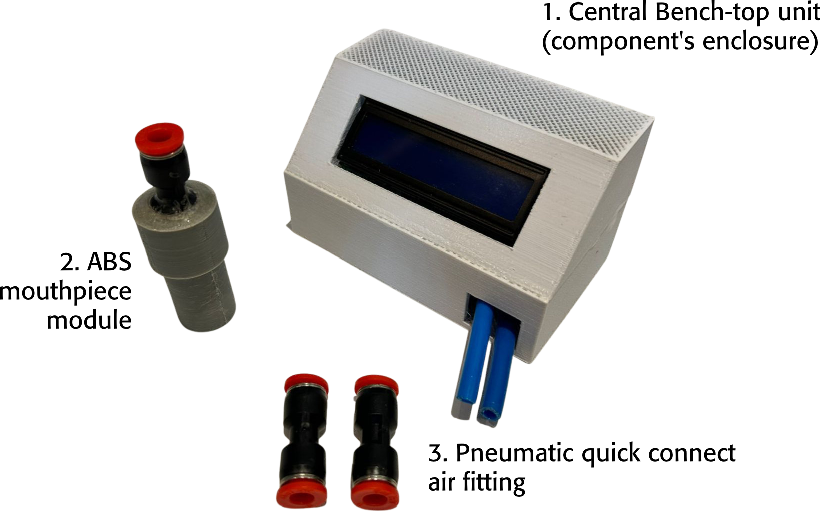
\includegraphics[width=\linewidth]{figures/3dppd_prototype.pdf}
  \caption{Photograph of the prototype, showing the central electronics module (top), the detachable mouthpiece module (left), and the air fitting connector (bottom).}
  \label{fig:3dppd_prototype}
\end{figure}

The modules are connected using pneumatic quick-connect air fittings (3 in Figure~\ref{fig:3dppd_prototype}) attached to the pressure sensor ports through pneumatic tubes of 4.9~mm diameter. These fittings reduce friction and the effort required for assembly and disassembly. The quick-connect design enables routine replacement of the user-contact module and streamlines cleaning procedures between assessments. Additionally, these connectors reduce the risk of contamination by limiting direct contact between the sensor ports and the replacement module.

To address varying usage scenarios, the mouthpiece module offers two configurations. The first is a reusable mouthpiece designed for repeated use with appropriate hygienization, featuring a 14.6 mm internal airway bore, a 25 mm base outer diameter, and an overall length of 49 mm. The second configuration is a cylindrical adapter that accommodates a disposable 23 mm cardboard mouthpiece, suitable for high-throughput clinical environments. This approach preserves a consistent sensing and processing pipeline while adapting the user-contact interface to practical requirements across diverse settings.

Figure~\ref{fig:3dppd_hw_simplified} presents the main components of the central unit. The module integrates an ESP32 microcontroller, a differential pressure sensor (MPX5500DP), and an LCD for local user feedback. The ESP32 is powered via its USB port and supplies power to peripheral components. The MPX5500DP is powered from the ESP32 5~V and GND rails, and its analog output (Vout) is conditioned before being sampled by an ESP32 analog input for analog-to-digital conversion (Table~\ref{tab:3dppd_hw_interfaces}). The sensor was selected for its broad operating range and for enabling differential pressure acquisition during inspiratory and expiratory maneuvers with a single sensing element. Reference values indicate that MIP values for healthy individuals typically range from -100 to -160~\ensuremath{\mathrm{cmH_2O}}, while MEP values range from 100 to 200~\ensuremath{\mathrm{cmH_2O}}~\cite{araujoReferenceValuesRespiratory2024}. 

\begin{figure*}[htp]
  \centering
  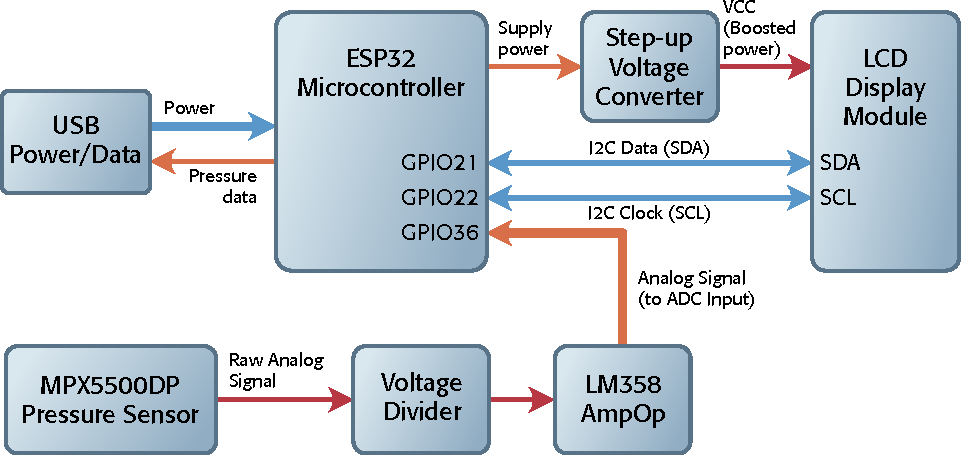
\includegraphics[width=0.6\linewidth]{figures/3dppd_hw_simplified.pdf}
  \caption{Simplified architecture and interfaces of 3D-PPD central module.}
  \label{fig:3dppd_hw_simplified}
\end{figure*}

The MPX5500DP produces an analog output proportional to the applied differential pressure. This signal is sampled by the ESP32 Analog-Digital Converter (ADC), and device-specific calibration converts the averaged ADC code into pressure values expressed in \ensuremath{\mathrm{cmH_2O}}.

Local user feedback is provided through an LCD equipped with an Inter-Integrated Circuit (I2C) interface module. A step-up module supplies the 5 V rail required by the LCD. The I2C interface connects to the ESP32 using GPIO 21 for SDA (data) and GPIO 22 for SCL (clock). Table~\ref{tab:3dppd_hw_interfaces} summarizes the primary hardware components and interfaces to provide a comprehensive overview of the hardware setup.

\begin{table}[htp]
  \centering
  \caption{Main components and interfaces of the prototype.}
  \label{tab:3dppd_hw_interfaces}
  \renewcommand{\arraystretch}{1.2}
  \begin{tabularx}{\columnwidth}{@{}lX@{}}
    \toprule
    \textbf{Component} & \textbf{Connection and role} \\
    \midrule
    ESP32 development board & USB-powered embedded controller responsible for sampling, calibration mapping, and communication with the host. \\
    
    \makecell[tl]{MPX5500DP differential\\ pressure sensor} & Powered from ESP32 5~V and GND; analog Vout attenuated via a resistive divider (68~k$\Omega$ to GND) and buffered by an LM358-based conditioning stage for sampling by an ESP32 ADC-capable input (SP/GPIO~36). \\
        
    \makecell[tl]{LM358 operational\\ amplifier module} & Analog signal-conditioning stage used to buffer the scaled sensor output prior to ADC sampling; includes a 68~k$\Omega$ (1/4~W) resistor to ground for voltage attenuation. \\
    
    LCD with I2C interface & Powered via a 5~V step-up stage; SDA connected to GPIO~21 and SCL connected to GPIO~22. \\
    \makecell[tl]{Pneumatic quick-connect\\ fittings} & Coupling of the mouthpiece module to the sensor ports for rapid replacement and cleaning. \\
    \bottomrule
  \end{tabularx}
\end{table}

\subsection{Data acquisition and device calibration}

Calibration is essential for ensuring data accuracy by establishing a reliable correlation between raw sensor readings and actual physical pressure values. During routine operation, the firmware samples the conditioned sensor output and applies multi-sample averaging to reduce signal acquisition noise. In the current implementation, each reported pressure value is calculated as the arithmetic mean of \(N=1000\) consecutive ADC readings. This averaging functions as a simple low-pass filter, minimizing the impact of high-frequency fluctuations on the signal.

The averaged ADC value is then converted into \ensuremath{\mathrm{cmH_2O}} using a device-specific calibration mapping embedded in the firmware, and the resulting data are transmitted to the desktop application via Bluetooth or USB. The integrated LCD also provides local user feedback by displaying status messages such as device readiness, connection status, and acquisition progress. The firmware operates in a continuous loop, with session boundaries managed by the desktop application. Algorithm~\ref{alg:3dppd_acquisition_flow} summarizes the runtime acquisition logic.


\begin{algorithm}[htp]
  \caption{3D-PPD data acquisition/transmission flow.}
  \label{alg:3dppd_acquisition_flow}
  \small
  \renewcommand{\baselinestretch}{1.3}
  \selectfont
    \begin{algorithmic}[1]
      \STATE Initialize UART, ADC input, Bluetooth interface, and LCD (I2C)
      \STATE Load device-specific calibration coefficients
      \STATE Display device-ready status on LCD
      \WHILE{true}
        \STATE Acquire \(N\) ADC readings and compute mean (\(N=1000\))
        \STATE Convert mean ADC code to pressure using calibration mapping
        \IF{Bluetooth connected}
          \STATE Transmit pressure value over Bluetooth
          \STATE Update LCD with acquisition status
          \STATE Delay 100~ms
        \ELSE
          \STATE Transmit pressure value via USB serial (wired mode)
          \STATE Update LCD with connection status
        \ENDIF
      \ENDWHILE
    \end{algorithmic}
\end{algorithm}

During data acquisition, pressures are reported in \ensuremath{\mathrm{cmH_2O}} according to the clinical sign convention, where negative values correspond to inspiratory maneuvers and positive values correspond to expiratory maneuvers.

Before clinical use, each prototype is calibrated offline to establish the mapping between averaged ADC codes and physical pressure values. Calibration is conducted using a screw-driven pneumatic pressure generator (Em\'{\i}lia) paired with a reference manometer (Famabras, Cidepe). The device is connected directly to the pressure source using tubing dimensions identical to those of the final prototype to minimize systematic errors resulting from pneumatic impedance or dead volume.

Data were collected at multiple discrete pressure levels up to 0.3~kgf/cm\textsuperscript{2} (approximately 300~\ensuremath{\mathrm{cmH_2O}}). At each setpoint, 200 averaged ADC samples were recorded and stored in a CSV file for regression analysis. {The calibration mapping embedded in the firmware was the mapping used during participant testing.} For the evaluated prototype, {this mapping was implemented as a device-specific empirical polynomial correction} (Equation~\ref{eq:poly_symbolic}), where \(x\) denotes the averaged ADC code and \(c_i\) are the fitted coefficients.

{This calibration mapping was intended to characterize the entire acquisition chain, including the pressure sensor, signal-conditioning stage, ESP32 analog-to-digital conversion, and pneumatic connections. Because empirical calibration models may be sensitive to boundary behavior, the assembled prototype was subsequently verified using independent pressure points measured with a water-filled U-tube manometer.}

\begin{equation}
\label{eq:poly_symbolic}
P(x) = \sum_{i=0}^{6} c_i x^i
\end{equation}

The coefficients \(c_0,\dots,c_6\) were embedded in the firmware for runtime conversion.

\subsection{Monitoring software}

The 3D-PPD supports both USB and Bluetooth communication modes between the embedded module and the desktop application. In the current prototype, the USB cable supplies power to the ESP32 and facilitates data transfer to the host computer. Bluetooth communication enables wireless operation when the device is powered by an outlet adapter. At the start of each evaluation session, the user selects the preferred communication mode in the desktop application, which then configures the acquisition pipeline accordingly.

The desktop application facilitates patient registration, guided assessment sessions, and retrospective analysis of previously recorded data. Patient information and evaluation results are stored in a local SQLite database, enabling fully offline operation. In addition to reporting numerical results for each assessment session, the application provides pressure--time visualizations for inspiratory and expiratory maneuvers, as well as a longitudinal view of repeated evaluations.

To support clinical workflows, the application organizes records by unique patient identifiers and associates each evaluation with a timestamp and repeated measurements for inspiratory and expiratory maneuvers. In the current implementation, each evaluation record includes three inspiratory and three expiratory measurements, enabling both within-session review and longitudinal comparison. The application also provides reference values derived from age- and sex-based prediction equations to contextualize recorded measurements during clinician review~\cite{araujoReferenceValuesRespiratory2024}.

Figure~\ref{fig:desktop_app_patient_history} shows the patient-history view used for longitudinal monitoring and retrieval of prior assessments. The screenshot is provided for illustration only and displays synthetic example data.

\begin{figure}[htp]
  \centering
  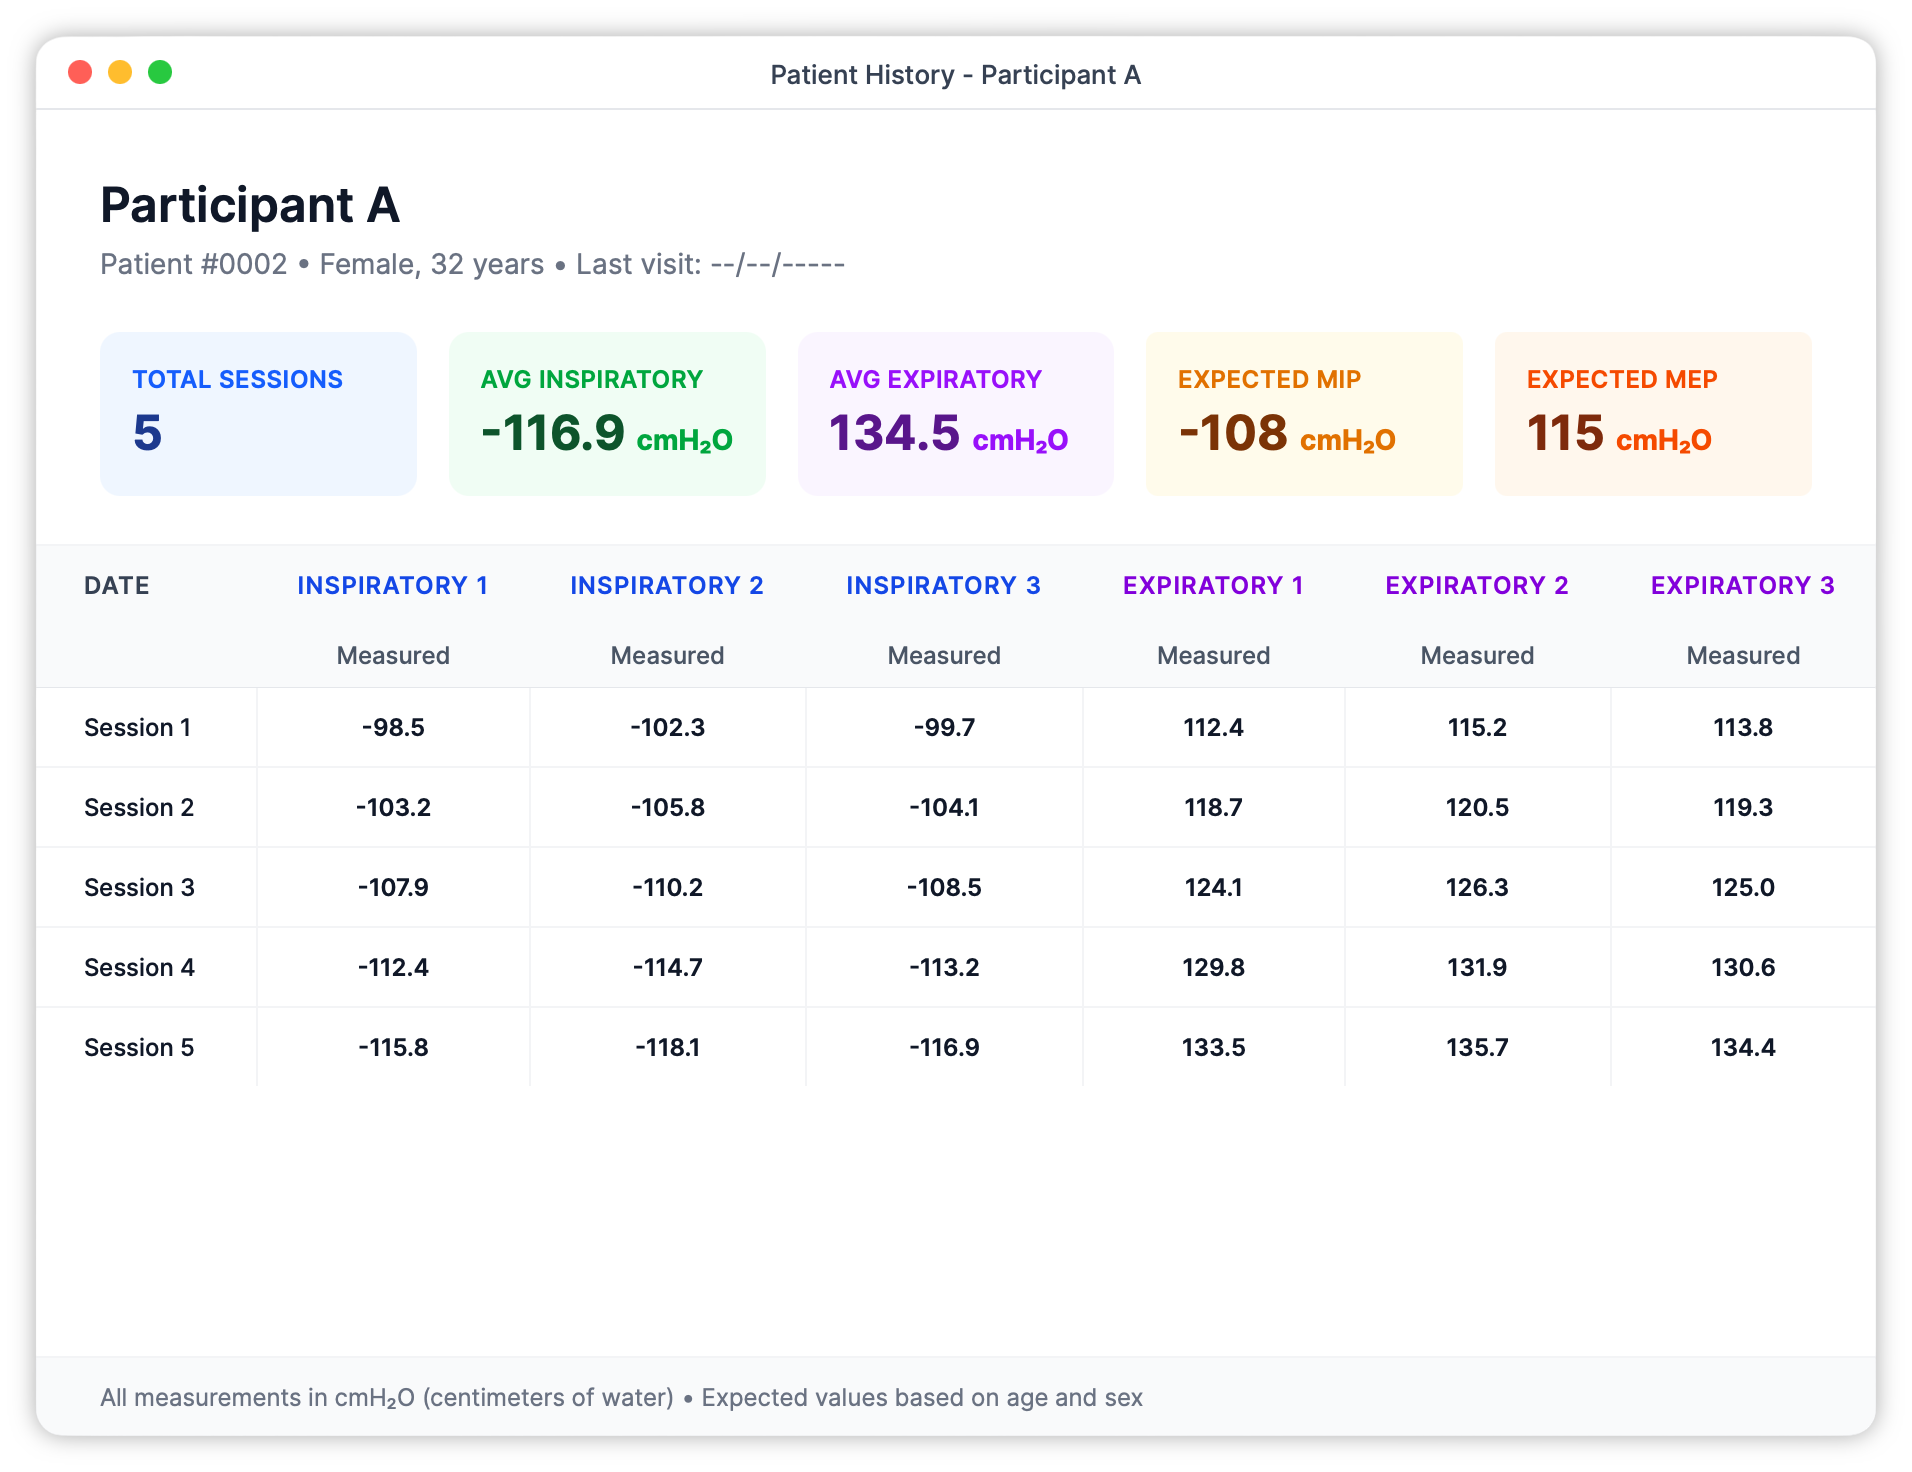
\includegraphics[width=\linewidth]{figures/desktop_app_patient_history.png}
  \caption{Patient-history view of the desktop application (synthetic example data). Each session stores three inspiratory and three expiratory trials and reports age- and sex-based expected values for contextualization.}
  \label{fig:desktop_app_patient_history}
\end{figure}

In practice, an assessment session consists of registering or selecting a patient record, choosing the communication mode, acquiring pressure traces for repeated inspiratory and expiratory maneuvers, and subsequently storing and reviewing the resulting measurements. The workflow is designed to ensure that the measurements remain traceable and retrievable over time while maintaining a lightweight data-handling pipeline suitable for resource-constrained environments.

\section{Validation Methodology}
\label{sec:validation_methodology}

This section describes the methodology and experimental protocol implemented to evaluate the assessment function of the proposed 3D-PPD. {{This study was designed as a pilot study to assess feasibility and provide a preliminary validation of the instrument’s psychometric properties. } Accordingly, a small convenience sample was recruited, in line with methodological recommendations for pilot studies. Content validity, concurrent validity in relation to a reference standard, and test–retest reliability of MIP and MEP measurements were emphasized.}

The protocol was developed to address three specific research questions:

\begin{description}
    \item[\textbf{RQ1}] Does the assessment workflow demonstrate adequate content validity as determined by expert review?
    \item[\textbf{RQ2}] Do MIP and MEP measurements obtained using the 3D-PPD correspond with those from a calibrated analog manovacuometer?
    \item[\textbf{RQ3}] Are MIP and MEP measurements reproducible within a single session and consistent across two evaluations conducted five days apart?
\end{description}

\subsection{Content validation}

Content validation assessed the relevance of the 3D-PPD for respiratory pressure measurement and the representativeness of its assessment workflow for MIP and MEP measurements~\cite{Souza2017,Yusoff2019}. A panel of six cardiopulmonary physiotherapists {specialized in cardiorespiratory physiotherapy, holding certification issued by the Brazilian Association of Respiratory Physiotherapy, Vascular Physiotherapy, and Intensive Care Physiotherapy (ASSOBRAFIR\textsuperscript{\textregistered}), were invited to participate as committee members. Access to potential expert panel members was obtained through the professional database available on the official ASSOBRAFIR\textsuperscript{\textregistered} website (https://assobrafir.com.br/). In this search, the filter “Bahia” was used under the “State” field, and ``Cardiorespiratory Physiotherapy'' under the ``Specialty'' field. A snowball sampling technique was also employed in the expert selection process. Thus, professionals who agreed to participate as committee members indicated other physiotherapists with specialist certification in the field of cardiorespiratory physiotherapy to take part in the study. After screening the candidates, the email address of each was identified through consultation of their Lattes CV via the Plataforma Lattes website (https://lattes.cnpq.br/). These email addresses were used to send invitations to participate as members of the expert panel, which evaluated the device in this stage of content validation. Therefore, the initial contact with the invited experts was made via email and included a brief introduction of the proposing research team, the study objectives, the steps to be undertaken after acceptance, and the link to the Informed Consent Form. The experts were blinded to the study hypotheses.}

After providing consent, the experts received a link to a presentation video produced by the research team. This video described the device workflow and demonstrated the assessment procedure, including the primary device components, connectivity options, and the monitoring software used during measurement sessions. The experts then evaluated the device using a researcher-developed questionnaire comprising five items and a four-point agreement scale (\emph{disagree}, \emph{neither disagree nor agree}, \emph{agree}, \emph{strongly agree}; coded from 1 to 4). {The inclusion of only five items in the questionnaire was a deliberate methodological choice, consistent with recommendations for content validation studies of technological devices. These items were selected because they cover the essential aspects of device performance, including measurement accuracy, assessment workflow functionality, usability, sealing/safety, and user comfort. This concise approach aimed to ensure an objective evaluation by experts, avoiding redundancy and response fatigue, while maintaining adequate coverage of the key domains required for device validation.} 

Content validation was conducted using a modified Delphi procedure~\cite{Souza2017,Yusoff2019} in two rounds. The device was refined between rounds based on expert feedback until a minimum consensus threshold of 70\% was achieved.

{The qualitative feedback provided by experts during the content validation process was systematically analyzed to guide iterative refinements of the device. Open-ended responses (“other considerations”) were independently reviewed by two researchers and analyzed using thematic content analysis. Similar comments were grouped into predefined domains, including usability, ergonomic design, device dimensions, and potential air leakage. Synthesized feedback was discussed by the research team, and when applicable, design modifications were implemented and directly linked to expert suggestions to ensure traceability. Decisions were based on technical feasibility, study objectives, and investigator consensus. Between Delphi rounds, the device was iteratively refined based on aggregated expert input until a minimum consensus threshold of 70\% was reached. When suggestions were not incorporated, methodological or technical justifications were recorded. This process ensured transparency and strengthened the robustness of the final device version.}

\subsection{Concurrent validation and reliability protocol}

To evaluate concurrent validity and reliability, participants aged 60 years or older of both sexes were recruited through convenience sampling. Eligibility criteria required independence in basic activities of daily living, defined as a Modified Barthel Index score of at least 50 points~\cite{Wang2022Comparison}, and independence in instrumental activities of daily living, defined as a Pfeffer Questionnaire score below 5 points~\cite{Dutra2015}. Individuals with pulmonary diseases or other chronic conditions that could prevent test execution were excluded. Participants who did not complete all scheduled evaluations were classified as lost to follow-up. The pilot study included 10 participants.

Maximal respiratory pressures were measured using two instruments: a previously calibrated analog manovacuometer, which served as the reference criterion, and the proposed 3D-PPD. All assessments were performed by the same assessor at two time points, with the second evaluation conducted five days after the first. The order of device use was randomized by numerical draw to minimize order effects. Identical instructions for respiratory maneuvers were provided for both devices.

For MIP assessment, participants were seated and fitted with a nasal clip. They were instructed to perform a maximal expiration outside the devices to reach residual volume, then to execute a maximal inspiratory effort through the device mouthpiece with lips sealed, sustaining the effort for two to three seconds. For MEP assessment, participants performed a maximal inspiration outside the devices to reach total lung capacity, followed by a maximal expiratory effort through the mouthpiece, also sustained for two to three seconds. Each maneuver was repeated three times, and the highest value was recorded. A one-minute rest was provided between maneuvers, or longer if necessary, until perceived exertion reached 6 points on the Borg scale~\cite{Borg1982}.

\subsection{Statistical analysis}

Statistical analyses were performed using SPSS (version 24.0, IBM Corp., Armonk, NY). Descriptive statistics were used to characterize the sample. Data normality was assessed through visual inspection (histograms and Q-Q plots) and the Shapiro-Wilk test. For data with normal distribution, continuous variables were reported as mean and standard deviation.

For content validity, the item-level content validity index (CVI) and the total CVI were calculated. Analysis of variance was applied to compare expert ratings between rounds~\cite{Yusoff2019}. CVI values were interpreted as inadequate if below 0.50, moderate if between 0.50 and 0.69, and high if between 0.70 and 1.00~\cite{Yusoff2019}.

In this study, item-level CVI was calculated as the proportion of experts who rated an item as either \emph{agree} or \emph{strongly agree} divided by the total number of experts. The item-level CVI is computed as shown in Equation~\ref{eq:icvi}, where \ensuremath{n^{(3,4)}_j} represents the number of experts who scored item \ensuremath{j} as 3 or 4, and \ensuremath{N_e} denotes the total number of experts.

\begin{equation}
  \mathrm{I\mbox{-}CVI}_j = \frac{n_j^{(3,4)}}{N_e}.
  \label{eq:icvi}
\end{equation}

The total CVI for the questionnaire is calculated according to Equation~\eqref{eq:scvi_ave} as the average of item-level CVI values across all \ensuremath{J} items.

\begin{equation}
  \mathrm{S\mbox{-}CVI/Ave} = \frac{1}{J}\sum_{j=1}^{J}\mathrm{I\mbox{-}CVI}_j.
  \label{eq:scvi_ave}
\end{equation}

To compare expert ratings between rounds, analysis of variance was conducted using the \ensuremath{F} statistic, as shown in Equation~\eqref{eq:anova_f}.

\begin{equation}
  F = \frac{\mathrm{MS}_{\mathrm{between}}}{\mathrm{MS}_{\mathrm{within}}},
  \label{eq:anova_f}
\end{equation}

\noindent where \ensuremath{\mathrm{MS}_{\mathrm{between}}} denotes the between-group mean square, and \ensuremath{\mathrm{MS}_{\mathrm{within}}} denotes the within-group mean square.

Concurrent validity was assessed by calculating the Intraclass Correlation Coefficient (ICC) between the 3D-PPD and the reference manovacuometer, while reliability was evaluated across the two time points using ICC. {A two-way mixed-effects model with absolute agreement was applied. Two approaches were considered: (1) the highest value obtained from repeated maneuvers, representing single-measure reliability (ICC[3,1]), and (2) the mean of three measurements, representing average-measure reliability (ICC[3,3]). This approach allows comparison between a clinically relevant scenario, based on the best effort, and a more stable estimate derived from averaged measurements. 95\% confidence intervals were calculated to estimate the precision of the reliability coefficients. This analysis was performed to determine the stability of measurements obtained by the same evaluator over time, accounting for potential systematic differences between repeated assessments.} ICC values were interpreted according to established thresholds: values above 0.75 indicate excellent reproducibility, values between 0.40 and 0.75 indicate reasonable to good reliability, and values below 0.40 indicate low reproducibility~\cite{Shrout1979}. 

{Agreement between devices was assessed using Bland–Altman analysis, including the calculation of mean bias (mean of the differences between the two methods), 95\% limits of agreement, and inspection for potential proportional bias (linear regression between the difference \mbox{\ensuremath{\text{Method A} - \text{Method B}}} and the mean of the methods \mbox{$\frac{(\text{A} + \text{B})}{2}$}.}
The statistical significance level was set at 5\% (p \textless 0.05).

For interpretability, ICC was expressed as variance components, where \ensuremath{\sigma^2_{\mathrm{sub}}} denotes the between-participant variance and \ensuremath{\sigma^2_{\mathrm{err}}} corresponds to the within-participant residual variance across repeated measurements. In this formulation, ICC is defined by Equation~\eqref{eq:icc_variance}.

\begin{equation}
  \mathrm{ICC} = \frac{\sigma^2_{\mathrm{sub}}}{\sigma^2_{\mathrm{sub}} + \sigma^2_{\mathrm{err}}}.
  \label{eq:icc_variance}
\end{equation}

\section{Results}
\label{sec:experimental_results}

This section reports the findings regarding calibration verification, content validity, concurrent validity, and reliability of maximal respiratory pressure measurements obtained with the proposed 3D-PPD and a reference manovacuometer.

The evaluation committee consisted of female experts in cardiorespiratory physiotherapy, with a median age of 42 years (range: 35 to 48 years) and a median of 19 years of clinical practice experience (range: 10 to 25 years). Five experts held a master's degree. After the first evaluation round, the device was revised based on expert feedback, including modifications to its dimensions and clarification of its functionality. The revised device was then evaluated in a second round by the same experts.

Table~\ref{tab:expert_ratings_rounds} summarizes the experts' ratings from both evaluation rounds. In the second round, items 3 to 5 achieved mean scores close to 4, indicating strong consensus regarding the software's user-friendliness, the efficient real-time capture and monitoring of information, and the 3D-PPD's effectiveness in fulfilling its assessment purpose.

\begin{table}[htp]
  \centering
  \caption{Means and standard deviations of experts' responses in the first and second rounds of analysis.}
  \label{tab:expert_ratings_rounds}
    \renewcommand{\arraystretch}{1.2}
    % Define Y to be a ragged-right version of X (improves readability for text)
    \newcolumntype{Y}{>{\raggedright\arraybackslash}X}
    
    % Setup: Left (fixed), Y (flexible), Center (fixed), Center (fixed)
    \begin{tabularx}{\columnwidth}{@{} l Y c c @{}}
    \toprule
    \textbf{Item} & \textbf{Content} & \makecell[c]{\textbf{1st round} \\\textbf{Mean} ($\sigma$)} &  \makecell[c]{\textbf{2nd round} \\\textbf{Mean} ($\sigma$)} \\
    \midrule
    1 & The dimensions of the 3D-PPD are suitable for its use. & 3.83 (0.40) & 3.16 (0.98) \\
    2 & The dimensions of the 3D-PPD are suitable for preventing air leakage during the evaluation maneuver. & 3.08 (0.90) & 3.00 (1.09) \\
    3 & The software that comes with the 3D-PPD is easy to use. & 3.50 (0.54) & 3.83 (0.40) \\
    4 & The information is captured quickly and can be viewed in real time on a computer or laptop. & 3.83 (0.40) & 3.83 (0.40) \\
    5 & The 3D-PPD fulfills its purpose of assessing respiratory pressures. & 3.50 (0.54) & 3.83 (0.40) \\
    \bottomrule
    \end{tabularx}
\end{table}

Table~\ref{tab:expert_cvi_rounds} presents item-level CVI values. In the second round, items 3 to 5 maintained high adequacy (item-level CVI of 1.00), while item 2 also demonstrated high adequacy. Item 1 remained lower than the others. The total CVI increased from 0.86 in the first round to 0.90 in the second round. An Analysis of Variance (ANOVA) for items 1 and 2 in the first round revealed a statistically significant difference among expert responses (p = 0.046), but this difference was not observed in the second round (p = 0.144), directly addressing RQ1.

{One item related to the device dimensions remained below the recommended threshold after the second Delphi round, with an item-level CVI of 0.66. This result indicates persistent variability in expert agreement regarding the ergonomic adequacy of the device, particularly in relation to its dimensions and potential implications for air leakage during use. Although consensus was achieved for the remaining items and the overall workflow was considered acceptable by the expert panel, this finding suggests that full agreement was not reached for all evaluated aspects. Therefore, while the general workflow was supported, the results highlight the need for further ergonomic refinements to optimize the device’s structural design prior to broader clinical implementation.}

\begin{table}[htp]
  \centering
  \caption{Item-level content validity index (CVI) in the first and second rounds of analysis.}
  \label{tab:expert_cvi_rounds}
  \renewcommand{\arraystretch}{1.2}
  % Define Y as a ragged-right X column for better text wrapping
  \newcolumntype{Y}{>{\raggedright\arraybackslash}X}
  
  % Column setup: Fixed, Flexible, Fixed, Fixed
  \begin{tabularx}{\columnwidth}{@{} l Y c c @{}}
    \toprule
    \textbf{Item} & \textbf{Content} & \textbf{1st round} & \textbf{2nd round} \\
    \midrule
    1 & The dimensions of the 3D-PPD are suitable for its use. & 0.66 & 0.66 \\
    2 & The dimensions of the 3D-PPD are suitable for preventing air leakage during the evaluation maneuver. & 0.66 & 0.83 \\
    3 & The software that comes with the 3D-PPD is easy to use. & 1.00 & 1.00 \\
    4 & The information is captured quickly and can be viewed in real time on a computer or laptop. & 1.00 & 1.00 \\
    5 & The 3D-PPD fulfills its purpose of assessing respiratory pressures. & 1.00 & 1.00 \\
    \bottomrule
\end{tabularx}
\end{table}

{To support the interpretation of the clinical validation analyses, the calibration behavior of the assembled prototype was verified using a water-filled U-tube manometer.} Ten positive-pressure levels (18--84.8~\ensuremath{\mathrm{cmH_2O}}) were applied, and device readings were compared to the physical reference calculated from the water column height difference ($P = \rho g \Delta h$). The results in Table~\ref{tab:calibration_results} show relative errors between the device and the reference ranging from 1.96\% to 8.8\%. The largest relative deviation occurred at the lowest pressure level, while errors at higher pressures remained below 4\%.

\begin{table}[htp]
  \centering
  \caption{Comparison between measured pressures and the respective percentage error relative to reference values.}
  \label{tab:calibration_results}
  
  \renewcommand{\arraystretch}{1.2}
  % Define Y as a ragged-right X column for better text wrapping
  \newcolumntype{Y}{>{\raggedright\arraybackslash}X}
  
  \begin{tabularx}{\columnwidth}{@{} Y Y Y @{}}
    \toprule
    \makecell[lt]{\textbf{Manometer}\\ (\ensuremath{\mathrm{cmH_2O}})} & 
    \makecell[lt]{\textbf{3D-PPD}\\ (\ensuremath{\mathrm{cmH_2O}})} & 
    \makecell[lt]{\textbf{Error}\\ (\%)} \\
    \midrule
    18.0 & 16.4145 & 8.8083 \\
    25.0 & 24.1245 & 3.5020 \\
    29.5 & 27.6385 & 6.3101 \\
    35.0 & 32.7919 & 6.3088 \\
    40.0 & 38.4393 & 3.9018 \\
    50.0 & 48.9335 & 2.1330 \\
    65.0 & 62.7885 & 3.4023 \\
    73.0 & 71.3836 & 2.2142 \\
    80.4 & 77.7777 & 3.2615 \\
    84.8 & 83.1393 & 1.9583 \\
    \bottomrule
  \end{tabularx}
\end{table}

{A complementary residual analysis was conducted using the same verification points to inspect whether the calibration error presented a systematic pattern across the tested range. Residuals were defined as the difference between the U-tube manometer reference pressure and the corresponding 3D-PPD pressure reading. \mbox{Figure~\ref{fig:calibration_residual_analysis}}(a) presents the residuals obtained during post-assembly verification. \mbox{Figure~\ref{fig:calibration_residual_analysis}}(b) shows the corresponding residual distribution.}

\begin{figure*}[htp]
  \centering

  \begin{minipage}[t]{0.45\linewidth}
    \centering
    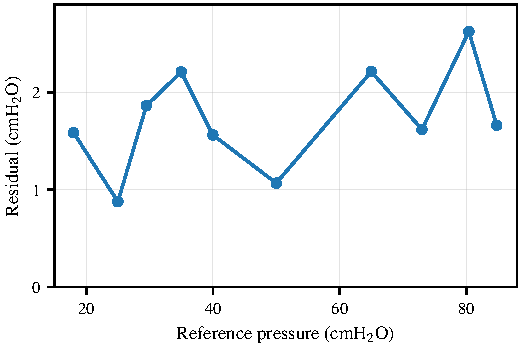
\includegraphics[width=\linewidth]{figures/fig_calibration_residuals.pdf}

    \vspace{0.3em}
    \small \textbf{(a)} {Residuals across the tested pressure range.}
    \label{fig:calibration_residuals}
  \end{minipage}
  \quad
  \begin{minipage}[t]{0.45\linewidth}
    \centering
    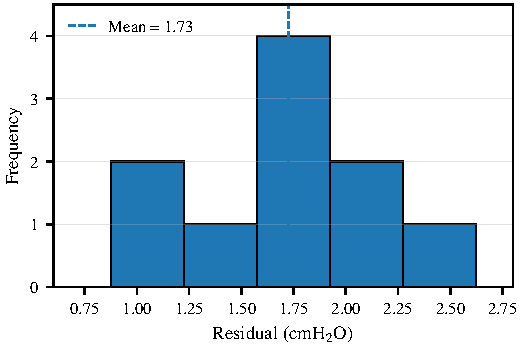
\includegraphics[width=\linewidth]{figures/fig_calibration_residual_distribution.pdf}

    \vspace{0.3em}
    \small \textbf{(b)} {Residual distribution analysis.}
    \label{fig:calibration_residual_distribution}
  \end{minipage}

  \caption{{Post-assembly calibration-verification analysis. Residuals were computed as the U-tube manometer reference pressure minus the 3D-PPD pressure reading.}}
  \label{fig:calibration_residual_analysis}
\end{figure*}

To assess concurrent validity and reliability, the pilot sample included 10 female participants aged 60 to 78 years, 80\% of whom identified as Black or Brown. Participants were randomly assigned to begin testing with either the manovacuometer (80\%) or the 3D-PPD (20\%). To address RQ2, Table~\ref{tab:concurrent_validity_icc} presents ICC values comparing 3D-PPD and manovacuometer measurements for MIP and MEP at both evaluation time points. Table~\ref{tab:within_session_repeatability} provides descriptive statistics for each trial within each evaluation and ICC results for each device. Table~\ref{tab:test_retest_reliability} displays test-retest ICC values between the first and second evaluations for the mean of the three trials and the highest value among trials, thus addressing RQ3. {ICC values were presented with their corresponding 95\% confidence intervals, allowing for an appropriate assessment of estimate precision and uncertainty.}

\begin{table*}[t] % 't' is usually better for double-column tables
  \centering
  \caption{ICC between 3D-PPD and manovacuometer measurements (concurrent validity). Values are reported in \ensuremath{\mathrm{cmH_2O}}.}
  \label{tab:concurrent_validity_icc}
  
  \renewcommand{\arraystretch}{1.2}
  
  % Custom column types
  \newcolumntype{Y}{>{\raggedright\arraybackslash}X}
  \newcolumntype{C}{>{\centering\arraybackslash}X}

  % Total columns = 5. Sum of coefficients: 1.4 + 1.1 + 1.1 + 0.9 + 0.5 = 5.0
  \begin{tabularx}{\linewidth}{@{}
    >{\hsize=1.4\hsize}Y  % Variable (Widest)
    >{\hsize=1.1\hsize}C  % 3D-PPD
    >{\hsize=1.1\hsize}C  % Manovacuometer
    >{\hsize=0.9\hsize}C  % ICC 
    >{\hsize=0.5\hsize}C  % p (Narrowest)
  @{}}
    \toprule
    \textbf{Variable} & \textbf{3D-PPD Mean} ($\sigma$) & \textbf{Manovacuometer Mean} ($\sigma$) & {\textbf{ICC ($\text{CI}_{95}$)}} & \textbf{p} \\
    \midrule
    
    \multicolumn{5}{@{}l}{\textbf{1st evaluation (MEP)}} \\
    Mean of 3 trials & 59.53 (16.19) & 51.66 (18.67) & {0.835 (0.326--0.959)} & 0.003 \\
    Highest value    & 65.21 (16.54) & 57.00 (20.57) & {0.718 (0.203--0.922)} & 0.003 \\
    \addlinespace 
    
    \multicolumn{5}{@{}l}{\textbf{1st evaluation (MIP)}} \\
    Mean of 3 trials & -56.89 (13.42) & -48.33 (11.46) & {0.827 (-0.134--0.964)} & \textless 0.001 \\
    Highest value    & -61.02 (14.65) & -55.00 (13.54) & {0.858 (0.150--0.970)} & \textless 0.001 \\
    \addlinespace
    
    \multicolumn{5}{@{}l}{\textbf{2nd evaluation (MEP)}} \\
    Mean of 3 trials & 59.94 (14.82) & 51.50 (12.08) & {0.886 (-0.085--0.971)} & \textless 0.001 \\
    Highest value    & 63.81 (15.17) & 57.50 (13.59) & {0.745 (0.227--0.931)} & 0.002 \\
    \addlinespace
    
    \multicolumn{5}{@{}l}{\textbf{2nd evaluation (MIP)}} \\
    Mean of 3 trials & -61.70 (16.68) & -51.83 (13.70) & {0.840 (-0.043--0.936)} & \textless 0.001 \\
    Highest value    & -61.13 (15.33) & -57.50 (16.87) & {0.764 (0.329--0.935)} & 0.003 \\
    \bottomrule
  \end{tabularx}
\end{table*}

Across both evaluation time points in Table~\ref{tab:concurrent_validity_icc}, ICC values ranged from 0.765 to 0.930 (all p \(\le\) 0.003), {indicating moderate-to-high correspondence between the 3D-PPD and the reference manovacuometer under the conditions of this pilot study, thereby addressing RQ2.}

\begin{table*}[htp]
  \centering
  \caption{Descriptive statistics and ICC results for repeated trials within each evaluation (reliability). Values are reported in \ensuremath{\mathrm{cmH_2O}}.}
  \label{tab:within_session_repeatability}
  
  \renewcommand{\arraystretch}{1.2}
  % Define 'C' as a Centered flexible column for the Headers/Means
  \newcolumntype{C}{>{\centering\arraybackslash}X}

  % Setup: 
  % Col 1: Fixed Left (Trials)
  % Col 2: Flexible Centered (3D-PPD Mean - allows header to wrap)
  % Cols 3-4: Fixed Center (ICC, p)
  % Col 5: Flexible Centered (Mano Mean - allows header to wrap)
  % Cols 6-7: Fixed Center (ICC, p)
  \begin{tabularx}{\textwidth}{@{} l C c c C c c @{}}
    \toprule
    & \multicolumn{3}{c}{\textbf{3D-PPD}} & \multicolumn{3}{c}{\textbf{Manovacuometer}} \\
    \cmidrule(lr){2-4} \cmidrule(l){5-7}
    \textbf{Variable} & \textbf{Mean} ($\sigma$) & {\textbf{ICC($\text{CI}_{95}$)}} & \textbf{p} & \textbf{Mean} ($\sigma$) & {\textbf{ICC ($\text{CI}_{95}$)}} & \textbf{p} \\
    \midrule
    
    % Group 1
    \multicolumn{2}{@{}l}{\textbf{1st evaluation (MEP)}} & {0.862 (0.665--0.960)} & \textless 0.001 & & {0.847 (0.614--0.956)} & \textless 0.001 \\
    Trial 1 & 60.60 (16.13) & & & 47.00 (20.57) & & \\
    Trial 2 & 60.81 (16.84) & & & 53.00 (14.94) & & \\
    Trial 3 & 57.19 (17.94) & & & 55.00 (22.23) & & \\
    \addlinespace
    
    % Group 2
    \multicolumn{2}{@{}l}{\textbf{2nd evaluation (MEP)}} & {0.858 (0.647--0.959)} & \textless 0.001 & & {0.704 (0.367--0.907)} & \textless 0.001 \\
    Trial 1 & 59.55 (16.68) & & & 52.50 (13.59) & & \\
    Trial 2 & 60.40 (15.50) & & & 50.50 (10.12) & & \\
    Trial 3 & 59.88 (14.68) & & & 51.50 (16.33) & & \\
    \addlinespace
    
    % Group 3
    \multicolumn{2}{@{}l}{\textbf{1st evaluation (MIP)}} & {0.834 (0.603--0.951)} & \textless 0.001 & & {0.635 (0.285--0.879)} & 0.001 \\
    Trial 1 & -54.21 (13.82) & & & -48.00 (11.35) & & \\
    Trial 2 & -59.59 (15.58) & & & -46.00 (9.66) & & \\
    Trial 3 & -56.88 (12.89) & & & -51.00 (17.28) & & \\
    \addlinespace
    
    % Group 4
    \multicolumn{2}{@{}l}{\textbf{2nd evaluation (MIP)}} & {0.931 (0.813--0.981)} & \textless 0.001 & & {0.761 (0.432--0.928)} & \textless 0.001 \\
    Trial 1 & -57.02 (14.79) & & & -47.50 (12.30) & & \\
    Trial 2 & -58.46 (13.69) & & & -51.50 (14.15) & & \\
    Trial 3 & -60.64 (15.26) & & & -56.50 (17.00) & & \\
\bottomrule
  \end{tabularx}
\end{table*}

\begin{table*}[t] % Changed to [t] for better top-of-page placement in two-column layouts
  \centering
  \caption{ICC between the first and second evaluations (test--retest reliability). Values are reported in \ensuremath{\mathrm{cmH_2O}}.}
  \label{tab:test_retest_reliability}
  
  \setlength{\tabcolsep}{3pt} 
  \renewcommand{\arraystretch}{1.2}
  
  \newcolumntype{C}{>{\centering\arraybackslash}X}
  
  \begin{tabularx}{\textwidth}{@{} 
    >{\hsize=1.4\hsize}X  % Variable
    >{\hsize=1.0\hsize}C  % 1st Eval (MEP)
    >{\hsize=1.0\hsize}C  % 2nd Eval (MEP)
    >{\hsize=1.2\hsize}C  % ICC (MEP) - Widened
    >{\hsize=0.6\hsize}C  % p (MEP) - Narrowed
    >{\hsize=1.0\hsize}C  % 1st Eval (MIP)
    >{\hsize=1.0\hsize}C  % 2nd Eval (MIP)
    >{\hsize=1.2\hsize}C  % ICC (MIP) - Widened
    >{\hsize=0.6\hsize}C  % p (MIP) - Narrowed
  @{}}
    \toprule
    & \multicolumn{4}{c}{\textbf{Maximum Expiratory Pressure (MEP)}} 
    & \multicolumn{4}{c}{\textbf{Maximum Inspiratory Pressure (MIP)}} \\
    \cmidrule(lr){2-5} \cmidrule(l){6-9}
    
    \textbf{Variable} 
    & \textbf{1st Eval} & \textbf{2nd Eval} & {\textbf{ICC ($\text{CI}_{95}$)}} & \textbf{p} 
    & \textbf{1st Eval} & \textbf{2nd Eval} & {\textbf{ICC ($\text{CI}_{95}$)}} & \textbf{p} \\
    \midrule
    
    \multicolumn{9}{@{}l}{\textbf{3D-PPD}} \\
    Mean of 3 trials & 59.53 (16.19) & 59.94 (14.82) & {0.938 (0.747--0.985)} & \textless 0.001 & -56.89 (13.42) & -61.70 (16.68) & {0.917 (0.628--0.980)} & \textless 0.001 \\
    Highest value    & 65.21 (16.54) & 63.81 (15.17) & {0.853 (0.518--0.961)} & 0.001           & -61.02 (14.65) & -61.13 (15.33) & {0.926 (0.728--0.981)} & \textless 0.001 \\
    \addlinespace
    
    \multicolumn{9}{@{}l}{\textbf{Manovacuometer}} \\
    Mean of 3 trials & 51.66 (18.67) & 51.50 (12.08) & {0.933 (0.724--0.983)} & \textless 0.001 & -48.33 (11.46) & -51.83 (13.70) & {0.898 (0.611--0.974)} & 0.001 \\
    Highest value    & 57.00 (20.57) & 57.50 (13.59) & {0.794 (0.352--0.945)} & 0.002           & -55.00 (13.54) & -57.50 (16.87) & {0.784 (0.119--0.946)} & 0.019 \\
    \bottomrule
  \end{tabularx}
\end{table*}

From the results presented in Tables~\ref{tab:within_session_repeatability} and~\ref{tab:test_retest_reliability}, within-session ICC values ranged from 0.846 to 0.940 and test--retest ICC values ranged from 0.843 to 0.918 . For the reference manovacuometer, within-session ICC values ranged from 0.635 to 0.875, and test--retest ICC values ranged from 0.629 to 0.862.

{Bland–Altman plots and mean bias with 95\% limits of agreement were presented in \mbox{Figures~\ref{fig:bland_altman_a}, \ref{fig:bland_altman_b}, \ref{fig:bland_altman_c}, and \ref{fig:bland_altman_d}}. No relevant proportional bias was observed between the devices (MEP 1st Assessment, \mbox{$\text{p}=0.341$}; MIP 1st Assessment, \mbox{$\text{p}=0.552$}; MEP 2nd Assessment, $\text{p}=0.612$; MIP 2nd Assessment, \mbox{$\text{p}=0.682$}).}

\begin{figure}
    \centering
    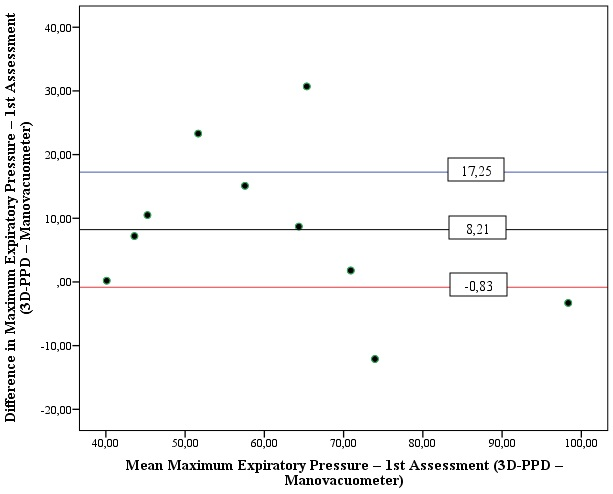
\includegraphics[width=1\linewidth]{figures/fig_bland_altman_1.jpg}
    \caption{Bland-Altman Plot indicating mean difference and 95\% limits of agreement between measurements from the 3D-PPD and Manovacuometer for Maximal Expiratory Pressure (1st assessment).}
    \label{fig:bland_altman_a}
\end{figure}

\begin{figure}
    \centering
    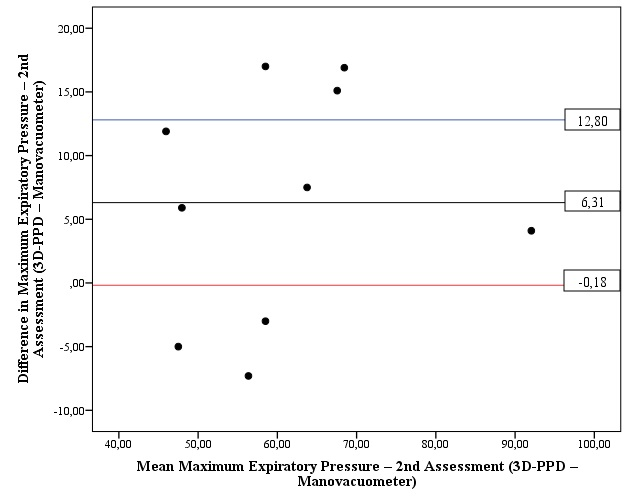
\includegraphics[width=1\linewidth]{figures/fig_bland_altman_2.jpg}
    \caption{Bland-Altman Plot indicating mean difference and 95\% limits of agreement between measurements from the 3D-PPD and Manovacuometer for Maximal Expiratory Pressure (2nd assessment).}
    \label{fig:bland_altman_b}
\end{figure}

\begin{figure}
    \centering
    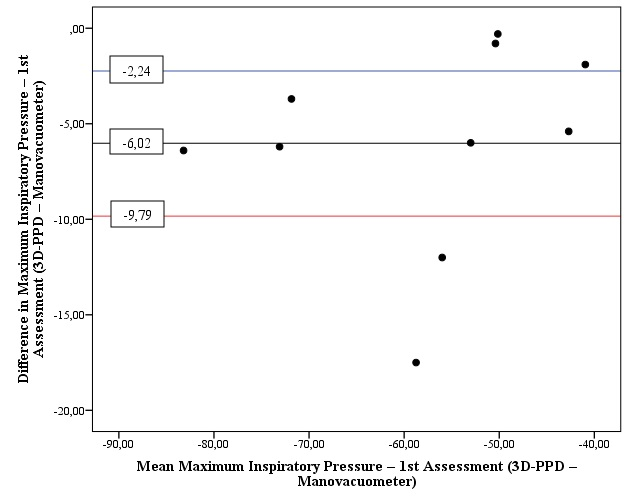
\includegraphics[width=1\linewidth]{figures/fig_bland_altman_3.jpg}
    \caption{Bland-Altman Plot indicating mean difference and 95\% limits of agreement between measurements from the 3D-PPD and Manovacuometer for Maximal Inspiratory Pressure (1st assessment).}
    \label{fig:bland_altman_c}
\end{figure}

\begin{figure}
    \centering
    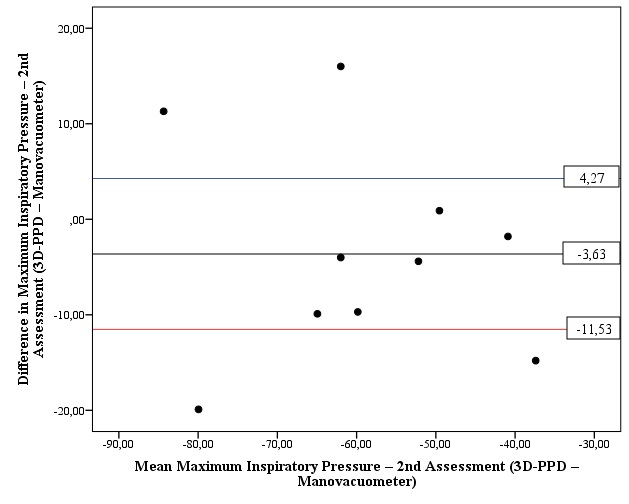
\includegraphics[width=1\linewidth]{figures/fig_bland_altman_4.jpg}
    \caption{Bland-Altman Plot indicating mean difference and 95\% limits of agreement between measurements from the 3D-PPD and Manovacuometer for Maximal Inspiratory Pressure (2nd assessment).}
    \label{fig:bland_altman_d}
\end{figure}

\section{Discussion and Practical Implications}
\label{sec:discussion}

Maximal respiratory pressures are widely utilized in respiratory physiotherapy and pulmonology to inform clinical reasoning for diagnosis, monitor rehabilitation interventions, and guide decisions regarding ventilatory support~\cite{Silveira2024Reliability}. Within this framework, the present study evaluated the proposed 3D-PPD in terms of content validity, concurrent validity relative to a reference manovacuometer, and the reliability of MIP and MEP measurements.

{The post-assembly calibration verification provides additional evidence on the behavior of the measurement chain. The observed deviations were larger at the lowest positive-pressure point and smaller across the remaining verification range, indicating that calibration uncertainty was more pronounced near the lower boundary of the tested interval. This finding reinforces the importance of reporting residual behavior alongside global fit indices in future calibration protocols. It also indicates that subsequent device iterations should prospectively validate calibration stability across broader positive and negative pressure ranges, particularly because MIP and MEP measurements involve opposite pressure directions.}

The content validation results indicate that the assessment workflow is generally well aligned with the intended construct. The total CVI increased from 0.86 in the first round to 0.90 in the second round (Table~\ref{tab:expert_cvi_rounds}). Items related to the software, information capture, and assessment purpose maintained item-level CVI values of 1.00 across both rounds. However, the item concerning device dimensions remained at 0.66, highlighting the need for further refinement of ergonomic aspects and user-interface geometry. Expert feedback also identified a practical concern regarding the air outlet design and its potential to interfere with maneuver execution, underscoring the importance of minimizing air leakage and preventing compensatory behavior during maximal efforts.

From a device design perspective, these findings indicate that current limitations are primarily associated with the user-device interface rather than the measurement objective. Maximal pressure testing is sensitive to factors such as mouthpiece sealing, glottic closure, and maneuver standardization. Consequently, small mechanical details, including mouthpiece geometry and the presence of a controlled leak or outlet, can influence both feasibility and measurement quality. Future iterations should prioritize redesigning the mouthpiece module to incorporate features that facilitate standardized maneuvers, such as a small leak or outlet consistent with established respiratory muscle testing practices. Subsequent evaluations should then determine whether the dimensions-related item aligns with the remaining items following these revisions~\cite{ATS2002,silveiraNewMethodMaximalPressures2021}.

In addition to measurement outcomes, the device architecture has important implications for implementation and iterative development. As detailed in Section~\ref{sec:3dppd_architecture_design}, the prototype separates the central module from a detachable mouthpiece module. This design facilitates hygienization and replacement of user-contact components in multi-user environments. The modularity also enables targeted modifications to the mouthpiece geometry, as highlighted by the dimensions-related item, without necessitating changes to the sensing and acquisition pipeline.

{Regarding usability, the software was rated favorably by the expert panel, particularly for perceived ease of use. This result was obtained as part of the expert-based content-validation process and does not constitute a formal usability study. Therefore, the findings support only a preliminary indication of perceived usability from expert opinion. In the current implementation, the software records the complete pressure--time trajectory and reports the highest value after three attempts, which may reduce misinterpretation during the maneuver and enhance traceability of the assessment session. Future evaluations should include structured usability protocols, involving clinicians and potential users, to quantify the usability, learnability, and workflow integration of the software using validated instruments for eHealth applications~\mbox{\cite{Maramba2019}}.}

Furthermore, integrating a digital pressure trace with automatic selection of summary values {creates opportunities for future quality-control procedures that are more difficult to implement with analog instruments.} For instance, trace-level checks, such as detecting abrupt leaks, insufficient plateau duration, or inconsistent effort patterns across trials, could be incorporated into the acquisition workflow to identify maneuvers requiring repetition. Although these mechanisms were not evaluated in the present study, they represent a {potential direction for improving measurement documentation and trial-review procedures in future versions of the system.}

{The inclusion of only {10} apparently healthy older women limits external validity and constrains the generalizability of the findings to broader and clinically heterogeneous populations. The small and homogeneous sample may have influenced ICC estimates, given that restricted between-subject variability can compromise the stability of variance components and lead to potentially inflated reliability coefficients. {In addition, some ICC estimates presented wide confidence intervals, reflecting the uncertainty associated with the limited sample size}.}

{{Another limitation of this study is the absence of calibration across the full clinically relevant range of negative and positive pressures associated with MIP and MEP measurements, as well as the lack of inter-rater reliability assessment, as all measurements were performed by a single assessor.} This prevents evaluation of the reproducibility of the results across different clinicians, which is particularly relevant for devices intended for clinical application. Therefore, future studies should include multiple assessors to investigate the robustness of the measurements across different operators.

{Thus, the present results should be considered as preliminary evidence of feasibility and validity, and further studies with larger, more diverse samples are needed to confirm the device's clinical performance.}

\section{Conclusion}
\label{sec:conclusion}
%
This {pilot} study introduced a low-cost, modular 3D-printed portable device (3D-PPD) for maximal respiratory pressure assessment. The system integrates a detachable mouthpiece module with a portable sensing and communication unit, enabling pressure--time data acquisition with local visualization and storage. Beyond detailing the device architecture and calibration workflow, the investigation examined three preliminary validation dimensions, focusing on expert-driven content validation of the assessment workflow, concurrent validity against a reference manovacuometer, and reliability across repeated trials and evaluation sessions.

{The expert review suggested that the proposed workflow was generally adequate for the intended assessment purpose after incremental refinement, although feedback on device dimensions indicates that the user--device interface still requires improvement. Pilot measurements also showed moderate-to-high correspondence between the 3D-PPD and the reference manovacuometer, as well as consistent repeated measurements under the tested protocol.} These findings provide preliminary evidence that digital traceability may be useful for documenting maximal-pressure assessment sessions and retrieving longitudinal records.

Nevertheless, the current evidence must be considered within the context of the study's limitations. The evaluation was conducted as a pilot study in a single setting, with a limited and homogeneous participant sample, and used an analog manovacuometer as the reference criterion. Furthermore, the investigation focused exclusively on the assessment function, without evaluating training-oriented capabilities. The measurement pipeline also relies on device-specific calibration and assembly details, which may affect generalizability across independently fabricated units. {Although post-assembly verification was added to characterize calibration behavior, this analysis covered only a limited positive-pressure range. Future prototypes should therefore incorporate prospectively defined calibration procedures with residual analysis, repeated post-assembly verification, and validation across both inspiratory and expiratory pressure domains.}

{Future research should prioritize larger, more diverse validation studies that include broader age groups, sexes, and clinical conditions, preferably with additional reference instrumentation when available. From a system-development perspective, subsequent iterations should refine the user--device interface to improve standardization of maneuvers and formalize trace-level quality-control criteria for trial acceptance or repetition. Transparent documentation of calibration artifacts, data-logging formats, software components, and assembly parameters would further support reproducibility and facilitate rigorous multi-site evaluation. Finally, although not evaluated in this study, the system could be extended to support remotely supervised home-based assessment or training workflows, contingent on dedicated validation of safety, usability, data security, and clinical effectiveness.}

{These results should be interpreted as preliminary and exploratory. Further studies involving larger, sex-balanced, and clinically diverse samples are required to establish more robust, stable, and generalizable estimates of the instrument’s psychometric properties.}

\section*{Declaration of interest statement}

The authors have no relevant financial or non-financial interests to disclose.

\section*{Ethics approval}

This study was performed in line with the principles of the Declaration of Helsinki. Approval was granted by the Ethics Committee of Federal University of Bahia (Date: 10/13/2022 / Number 5.698.604)

\section*{Concent to participate}

Informed consent was obtained from all individual participants included in the study.

%\section*{Acknowledgment}



% \bibliographystyle{IEEEtran}
% \bibliography{IEEEabrv,references}

% Generated by IEEEtran.bst, version: 1.14 (2015/08/26)
\begin{thebibliography}{10}
\providecommand{\url}[1]{#1}
\csname url@samestyle\endcsname
\providecommand{\newblock}{\relax}
\providecommand{\bibinfo}[2]{#2}
\providecommand{\BIBentrySTDinterwordspacing}{\spaceskip=0pt\relax}
\providecommand{\BIBentryALTinterwordstretchfactor}{4}
\providecommand{\BIBentryALTinterwordspacing}{\spaceskip=\fontdimen2\font plus
\BIBentryALTinterwordstretchfactor\fontdimen3\font minus \fontdimen4\font\relax}
\providecommand{\BIBforeignlanguage}[2]{{%
\expandafter\ifx\csname l@#1\endcsname\relax
\typeout{** WARNING: IEEEtran.bst: No hyphenation pattern has been}%
\typeout{** loaded for the language `#1'. Using the pattern for}%
\typeout{** the default language instead.}%
\else
\language=\csname l@#1\endcsname
\fi
#2}}
\providecommand{\BIBdecl}{\relax}
\BIBdecl

\bibitem{labakiChronicRespiratoryDiseases2020}
W.~W. Labaki and M.~K. Han, ``Chronic respiratory diseases: A global view,'' \emph{The Lancet Respiratory Medicine}, vol.~8, no.~6, pp. 531--533, Jun. 2020.

\bibitem{merhejEpidemiologyAsthmaPrevalence2023}
T.~Merhej and J.~G. Zein, ``Epidemiology of {{Asthma}}: {{Prevalence}} and {{Burden}} of {{Disease}},'' in \emph{Precision {{Approaches}} to {{Heterogeneity}} in {{Asthma}}}, ser. Advances in {{Experimental Medicine}} and {{Biology}}, A.~R. Brasier and N.~N. Jarjour, Eds.\hskip 1em plus 0.5em minus 0.4em\relax Cham: Springer International Publishing, 2023, pp. 3--23.

\bibitem{Spruit2013}
C.~K. Lan, L.~Nici, and R.~Z. Wallack, ``Pulmonary {{Rehabilitation}},'' \emph{COPD}, vol. 188, pp. 167--190, Oct. 2010.

\bibitem{Holland2021}
A.~E. Holland, N.~S. Cox, L.~{Houchen-Wolloff}, C.~L. Rochester, C.~Garvey, R.~ZuWallack, L.~Nici, T.~Limberg, S.~C. Lareau, B.~P. Yawn, M.~Galwicki, T.~Troosters, M.~Steiner, R.~Casaburi, E.~Clini, R.~S. Goldstein, and S.~J. Singh, ``Defining {{Modern Pulmonary Rehabilitation}}. {{An Official American Thoracic Society Workshop Report}},'' \emph{Annals of the American Thoracic Society}, vol.~18, no.~5, pp. e12--e29, May 2021.

\bibitem{Sanchez2023}
Z.~{S{\'a}nchez-Mil{\'a}}, V.~{Abu{\'i}n-Porras}, C.~{Romero-Morales}, J.~{Almaz{\'a}n-Polo}, and J.~Vel{\'a}zquez~Saornil, ``Effectiveness of a respiratory rehabilitation program including an inspiration training device {\emph{versus}} traditional respiratory rehabilitation: A randomized controlled trial,'' \emph{PeerJ}, vol.~11, p. e16360, Dec. 2023.

\bibitem{Belman1988}
M.~J. Belman and R.~Shadmehr, ``Targeted resistive ventilatory muscle training in chronic obstructive pulmonary disease,'' \emph{Journal of Applied Physiology}, vol.~65, no.~6, pp. 2726--2735, Dec. 1988.

\bibitem{Gohl2016}
O.~G{\"o}hl, D.~Walker, S.~Walterspacher, D.~Langer, C.~Spengler, T.~Wanke, M.~Petrovic, R.-H. Zwick, S.~Stieglitz, R.~Gl{\"o}ckl, D.~Dellweg, and H.-J. Kabitz, ``{Atemmuskeltraining: State-of-the-Art},'' \emph{Pneumologie}, vol.~70, no.~01, pp. 37--48, Jan. 2016.

\bibitem{Rietberg2017}
M.~B. Rietberg, J.~Veerbeek, E.~E. {van Wegen}, R.~Gosselink, and G.~Kwakkel, ``Respiratory muscle training for multiple sclerosis,'' \emph{Cochrane Database of Systematic Reviews}, vol. 2017, Nov. 2011.

\bibitem{vermaCapacityneedGapHospital2020}
V.~R. Verma, A.~Saini, S.~Gandhi, U.~Dash, and S.~F. Koya, ``Capacity-need gap in hospital resources for varying mitigation and containment strategies in {{India}} in the face of {{COVID-19}} pandemic,'' \emph{Infectious Disease Modelling}, vol.~5, pp. 608--621, Jan. 2020.

\bibitem{boroBarriersCOVID19Health2022}
E.~Boro and B.~Stoll, ``Barriers to {{COVID-19 Health Products}} in {{Low-and Middle-Income Countries During}} the {{COVID-19 Pandemic}}: {{A Rapid Systematic Review}} and {{Evidence Synthesis}},'' \emph{Frontiers in Public Health}, vol.~10, 2022.

\bibitem{pinnockImplementationDigitalHome2023}
H.~Pinnock, C.~Y. Hui, and J.~F.~M. {van Boven}, ``Implementation of digital home monitoring and management of respiratory disease,'' \emph{Current Opinion in Pulmonary Medicine}, vol.~29, no.~4, p. 302, Jul. 2023.

\bibitem{bosnic-anticevichAdvancingDigitalSolutions2023}
S.~{Bosnic-Anticevich}, N.~D. Bakerly, H.~Chrystyn, M.~Hew, and J.~van~der Palen, ``Advancing {{Digital Solutions}} to {{Overcome Longstanding Barriers}} in {{Asthma}} and {{COPD Management}},'' \emph{Patient Preference and Adherence}, vol.~17, pp. 259--272, Jan. 2023.

\bibitem{sepiacciSystematicReviewMetaAnalysis2025}
A.~Sepiacci, N.~Starc, R.~Laitano, F.~Pasqua, P.~Rogliani, and J.~Ora, ``Systematic {{Review}} and {{Meta-Analysis}} of the {{Application}} of {{T-PEP}} in the {{Therapeutic Management}} of {{COPD Patients}},'' \emph{Journal of Clinical Medicine}, vol.~14, no.~2, p. 320, Jan. 2025.

\bibitem{Pegoraro2018}
L.~G. d.~O. Pegoraro, R.~Gvozd, M.~d. C. F.~L. Haddad, M.~T.~O. Vannuchi, L.~G. d.~C. Silva, and M.~A. Rossaneis, ``Validation of instrument to assess software of patients' risk classification,'' \emph{Revista Brasileira de Enfermagem}, vol.~71, no.~3, pp. 975--982, May 2018.

\bibitem{paivaInspiratoryMuscleTraining2015}
D.~N. Paiva, L.~B. Assmann, D.~F. Bordin, R.~Gass, R.~T. Jost, M.~{Bernardo-Filho}, R.~A. Fran{\c c}a, and D.~M. Cardoso, ``Inspiratory muscle training with threshold or incentive spirometry: {{Which}} is the most effective?'' \emph{Revista Portuguesa de Pneumologia (English Edition)}, vol.~21, no.~2, pp. 76--81, Mar. 2015.

\bibitem{fernandez-lazaroInspiratoryMuscleTraining2021}
D.~{Fern{\'a}ndez-L{\'a}zaro}, D.~{Gallego-Gallego}, L.~Corchete, D.~Fern{\'a}ndez~Zoppino, J.~{Gonz{\'a}lez-Bernal}, B.~Garc{\'i}a~G{\'o}mez, and J.~{Mielgo-Ayuso}, ``Inspiratory {{Muscle Training Program Using}} the {{PowerBreath}}\textregistered : {{Does It Have Ergogenic Potential}} for {{Respiratory}} and/or {{Athletic Performance}}? {{A Systematic Review}} with {{Meta-Analysis}},'' \emph{International Journal of Environmental Research and Public Health}, vol.~18, no.~13, p. 6703, Jun. 2021.

\bibitem{araujoReferenceValuesRespiratory2024}
P.~R.~S. Ara{\'u}jo, J.~D. M.~D. Fonseca, A.~A. Marcelino, M.~A. Moreno, A.~D.~F. Dornelas De~Andrade, M.~O. Ya{\~n}ez, R.~{Torres-Castro}, V.~R. Resqueti, and G.~A. D.~F. Fregonezi, ``Reference values for respiratory muscle strength and maximal voluntary ventilation in the {{Brazilian}} adult population: {{A}} multicentric study,'' \emph{PLOS ONE}, vol.~19, no.~11, p. e0313209, Nov. 2024.

\bibitem{Souza2017}
A.~C. de~Souza, N.~M.~C. Alexandre, E.~d.~B. Guirardello, A.~C. de~Souza, N.~M.~C. Alexandre, and E.~d.~B. Guirardello, ``{Propriedades psicom\'etricas na avalia\c c\~ao de instrumentos: avalia\c c\~ao da confiabilidade e da validade},'' \emph{Epidemiologia e Servi\c cos de Sa\'ude}, vol.~26, no.~3, pp. 649--659, Jul. 2017.

\bibitem{Duckworth2011}
A.~L. Duckworth and M.~L. Kern, ``A meta-analysis of the concurrent validity of self-control measures,'' \emph{Journal of Research in Personality}, vol.~45, no.~3, pp. 259--268, Jun. 2011.

\bibitem{Nunnally1994}
{\relax CJ}.~Nunnally and I.~Bernstein, \emph{Psychometric Theory}, 3rd~ed.\hskip 1em plus 0.5em minus 0.4em\relax New York: McGraw-Hill, 1994.

\bibitem{pereiraTrueForceDigital2021}
M.~C.~B. Pereira, B.~M.~F. Silveira, H.~L.~A. Pereira, V.~F. Parreira, and H.~R. Martins, ``Trueforce: A new digital manometer to measure maximal respiratory pressures at functional residual capacity,'' \emph{Research on Biomedical Engineering}, vol.~37, no.~2, pp. 181--191, 2021.

\bibitem{silveiraNewMethodMaximalPressures2021}
B.~M.~F. Silveira, M.~C.~B. Pereira, D.~R. Cardoso, G.~A. Ribeiro-Samora, H.~R. Martins, and V.~F. Parreira, ``New method for evaluating maximal respiratory pressures: Concurrent validity, test-retest, and inter-rater reliability,'' \emph{Brazilian Journal of Physical Therapy}, vol.~25, no.~6, pp. 741--748, 2021.

\bibitem{silveiraMaximalPressuresFRC2023}
B.~M.~F. Silveira, H.~R. Martins, G.~A. Ribeiro-Samora, L.~F. Oliveira, E.~V. Mancuzo, M.~Velloso, and V.~F. Parreira, ``Maximal respiratory pressures: Measurements at functional residual capacity in individuals with different health conditions using a digital manometer,'' \emph{Brazilian Journal of Physical Therapy}, vol.~27, no.~4, p. 100529, 2023.

\bibitem{aguilarZambranoUbicu2025}
J.~Aguilar-Zambrano, E.~C. Wilches-Luna, H.~Asencio-Santofimio, M.~Valencia, D.~Riveros, A.~Navarro, J.~C. Martinez, E.~Tamura, J.~A. Loaiza, J.~Hernandez, D.~Sanchez, J.~D. Garcia, L.~Arzayus-Pati{\~n}o, V.~Perez-Hortua, E.~Moncada, and M.~Ram{\'i}rez, ``{{UBICU}}: A gamified respiratory incentive system for pulmonary re-expansion,'' \emph{IEEE Access}, vol.~13, pp. 15\,244--15\,252, 2025.

\bibitem{polancoBiomedicalEquipmentUbicu2024}
J.~J.~G. Polanco, I.~G. Mej{\'i}a, J.~A. Zambrano, M.~Valencia, E.~C. Moncada, and J.~D. Garcia, ``Biomedical equipment for the measurement of inspiratory and expiratory volumes based on the ubicu respiratory incentive,'' in \emph{2024 3rd International Congress of Biomedical Engineering and Bioengineering (CIIBBI)}, 2024, pp. 1--5.

\bibitem{sankarGaneshIncentiveSpirometry2024}
A.~Sankar~Ganesh, K.~Abathsagayam, and N.~P. Ravisankar, ``Impact of volume-oriented incentive spirometry on lung volume and peak expiratory flow rate in patients with tracheostomy,'' \emph{Cureus}, vol.~16, no.~3, p. e56820, 2024.

\bibitem{ndiayeIoTWakeCOVID192020}
M.~Ndiaye, S.~S. Oyewobi, A.~M. {Abu-Mahfouz}, G.~P. Hancke, A.~M. Kurien, and K.~Djouani, ``{{IoT}} in the {{Wake}} of {{COVID-19}}: {{A Survey}} on {{Contributions}}, {{Challenges}} and {{Evolution}},'' \emph{IEEE Access}, vol.~8, pp. 186\,821--186\,839, 2020.

\bibitem{dhruveAssessingAdherenceInhaled2022}
H.~Dhruve and D.~J. Jackson, ``Assessing adherence to inhaled therapies in asthma and the emergence of electronic monitoring devices,'' \emph{European Respiratory Review}, vol.~31, no. 164, Jun. 2022.

\bibitem{kimApplicationInternetMedical2022}
B.~Kim, S.~Kim, M.~Lee, H.~Chang, E.~Park, and T.~Han, ``Application of an {{Internet}} of {{Medical Things}} ({{IoMT}}) to {{Communications}} in a {{Hospital Environment}},'' \emph{Applied Sciences}, vol.~12, no.~23, p. 12042, Jan. 2022.

\bibitem{moraisIoTBasedWearableSmart2023}
D.~F.~T. Morais, G.~Fernandes, G.~D. Lima, and J.~J. P.~C. Rodrigues, ``{{IoT-Based Wearable}} and {{Smart Health Device Solutions}} for {{Capnography}}: {{Analysis}} and {{Perspectives}},'' \emph{Electronics}, vol.~12, no.~5, p. 1169, Jan. 2023.

\bibitem{Polit2006}
D.~F. Polit and C.~T. Beck, ``The content validity index: {{Are}} you sure you know what's being reported? critique and recommendations,'' \emph{Research in Nursing \&amp; Health}, vol.~29, no.~5, pp. 489--497, 2006.

\bibitem{Maramba2019}
I.~Maramba, A.~Chatterjee, and C.~Newman, ``Methods of usability testing in the development of {{eHealth}} applications: {{A}} scoping review,'' \emph{International Journal of Medical Informatics}, vol. 126, pp. 95--104, Jun. 2019.

\bibitem{Yusoff2019}
{\relax MSB}.~Yusoff, ``{{ABC}} of {{Content Validation}} and {{Content Validity Index Calculation}},'' \emph{Education in Medicine Journal}, vol.~11, pp. 49--54, 2019.

\bibitem{Wang2022Comparison}
Y.-C. Wang, P.~Chang, Y.-M. Chen, Y.-C. Lee, S.-L. Huang, M.-H. Chen, and C.~Hsieh, ``Comparison of responsiveness of the barthel index and modified barthel index in patients with stroke,'' \emph{Disability and Rehabilitation}, vol.~45, pp. 1097 -- 1102, 2022.

\bibitem{Dutra2015}
M.~C. Dutra, R.~d.~S. Ribeiro, S.~B. Pinheiro, G.~F. de~Melo, and G.~d.~A. Carvalho, ``Accuracy and reliability of the Pfeffer Questionnaire for the Brazilian elderly population,'' \emph{Dementia \& Neuropsychologia}, vol.~9, no.~2, pp. 176--183, Jun. 2015.

\bibitem{Borg1982}
G.~A. Borg, ``Psychophysical bases of perceived exertion,'' \emph{Medicine \& Science in Sports \& Exercise}, vol.~14, no.~5, pp. 377--381, 1982.

\bibitem{Shrout1979}
P.~E. Shrout and J.~L. Fleiss, ``Intraclass correlations: {{Uses}} in assessing rater reliability.'' \emph{Psychological Bulletin}, vol.~86, no.~2, pp. 420--428, 1979.

\bibitem{Silveira2024Reliability}
B.~M.~F. Silveira, H.~L.~A. Pereira, G.~Chaves, D.~G.~C. Ho, and V.~F. Parreira, ``Reliability and validity of maximal respiratory pressures,'' \emph{Respiratory Care}, vol.~69, pp. 881 -- 890, 2024.

\bibitem{ATS2002}
T.~Maher, ``Faculty {{Opinions}} recommendation of {{American Thoracic Society}}/{{European Respiratory Society International Multidisciplinary Consensus Classification}} of the {{Idiopathic Interstitial Pneumonias}}. {{This}} joint statement of the {{American Thoracic Society}} ({{ATS}}), and the {{European Respiratory Society}} ({{ERS}}) was adopted by the {{ATS}} board of directors, {{June}} 2001 and by the {{ERS Executive Committee}}, {{June}} 2001.'' \emph{Faculty Opinions -- Post-Publication Peer Review of the Biomedical Literature}, vol. 166, pp. 518--624, Feb. 2014.

\end{thebibliography}


% --- Author 1: Giselle Bárbara de Almeida Scaldaferri ---
\begin{IEEEbiographynophoto}{Giselle B\'arbara de Almeida Scaldaferri}
is currently a Physiotherapist. Giselle received the B.S. degree in Physical Therapy from the Federal University of Bahia, Brazil in 2021 and the M.Sc. degree in Rehabilitation Sciences from the Federal University of Bahia, Brazil, in 2024. Her research interests include rehabilitation and technology.
\end{IEEEbiographynophoto}

% --- Author 2: Yuri Lima dos Santos Silva ---
\begin{IEEEbiographynophoto}{Yuri Lima dos Santos Silva}
received the B.S. degree in Exact and Technological Sciences from Federal University of Recôncavo da Bahia, Brazil in 2024. He is currently pursuing a B.S degree in Computer Engineering in Federal University of Recôncavo da Bahia, Brazil. His research interests include machine learning applications and embedded systems.
\end{IEEEbiographynophoto}

% --- Author 3: Vitória Caldas Lordelo de Brito ---
\begin{IEEEbiographynophoto}{Vit\'oria Caldas Lordelo de Brito}
is currently a Critical Care Physical Therapist at Hospital Ana Nery, Brazil. Vitória received the B.S. degree in Physical Therapy from the Federal University of Bahia (2024). Her research interests include rehabilitation and technology.
\end{IEEEbiographynophoto}

% --- Author 4: Matheus Sales ---
\begin{IEEEbiographynophoto}{Matheus Sales}
is currently a Professor at the Faculty of Physical Therapy at Santa Casa Faculty, Brazil. Matheus received the B.S. and M.Sc. degree in Interactive Processes of Organs and Systems from the Federal University of Bahia (2018-2023). His research interests include rehabilitation and technology.
\end{IEEEbiographynophoto}

% --- Author 5: Marcela Rodrigues de Castro ---
\begin{IEEEbiographynophoto}{Marcela Rodrigues de Castro}
is currently a Professor at the Faculty of Education at Federal University of Bahia, Brazil. Marcela received the B.S. degree in Physical Education Teaching from the Federal University of Juiz de Fora (2003), the M.Sc. degree in Physical Education from the Federal University of Juiz de Fora, in the research line "Sociocultural Aspects of Human Movement” (2009), and the Ph.D. in Movement Sciences, with a concentration in “Biodynamics of Human Movement,” from São Paulo State University (2014). Her research interests include rehabilitation and technology.
\end{IEEEbiographynophoto}

% --- Author 6: João Carlos N. Bittencourt ---
\begin{IEEEbiographynophoto}{Jo\~ao Carlos N. Bittencourt}
(M'15) is currently a Professor of the Center of Exact and Technological Sciences at Federal University of Recôncavo da Bahia, Brazil. João received the B.S. degree in Computer Engineering from the State University of Feira de Santana and the M.Sc. degree in Electrical Engineering from the Federal University of Bahia, Brazil, in 2013 and 2017. His research interests include the areas of embedded systems, digital design, Internet of Things, and smart cities.
\end{IEEEbiographynophoto}

% --- Author 7: João Soares de Oliveira Neto ---
\begin{IEEEbiographynophoto}{Jo\~ao Soares de Oliveira Neto}
received the B.S. degree in computer science from the Federal University of Maranhão, São Luís, Brazil, in 1999, the M.S. degree in computer science from the Federal University of Santa Catarina, Florianópolis, Brazil, in 2003, and the Ph.D. degrees in electrical engineering from the University of São Paulo, São Paulo, Brazil, and in computer science from the Université Paris-Saclay, France (double degree). He is currently an Associate Professor with the Federal University of Bahia, Salvador, Brazil. His research interests include human–computer interaction, accessibility, software engineering, ubiquitous computing, and the development of digital assistive technology for urban spaces.
\end{IEEEbiographynophoto}

% --- Author 8: Daniel Dominguez Ferraz ---
\begin{IEEEbiographynophoto}{Daniel Dominguez Ferraz}
is currently a Professor at the Multidisciplinary Institute of Rehabilitation and Health at Federal University of Bahia, Brazil. Daniel received the B.S. degree in Physical Therapy from the University of La Coruña (2005), the MSc. Degree in Neurorehabilitation from the Autonomous University of Barcelona (2008), and the Ph.D. in Health Sciences from the Federal University of Bahia (2018). His research interests include rehabilitation and technology.
\end{IEEEbiographynophoto}

\vfill
\EOD

\end{document}
